 % The main file for CAMP reports
 % Don't put any content in here. 
 % Don't even include content files by using \input or \inlcude. 
 % Put your content to TEXT.TEX or include it there using \input.
 % Uses:
 %		SETTINGS.TEX	contains the settings for this document
 %		COMMANDS.TEX	contains commands which can be used while writing
 %		INFO.TEX			contains the author, title and so on for the cover
 %		COVER.TEX			formats the front cover of the document
 %		ABSTRACT.TEX	contains the abstract to be included (if needed)
 %		TEXT.TEX			contains the actual content of the document
 %		BIB.BIB				containt the BibTeX entries for the document
 
 
%% Draft document mode
%% Final document
\documentclass[12pt,a4paper,bibtotoc,idxtotoc,headsepline,footsepline,footexclude,BCOR12mm,DIV13]{scrbook}
\usepackage[bindingoffset=0.2in,left=1.2in,right=1.2in,top=1.8in,bottom=1.2in,footskip=.5in]{geometry}
%\documentclass[11pt,a4paper,bibtotoc,idxtotoc,headsepline,footsepline,footexclude,BCOR20mm,DIV10]{scrbook}

% KOMA-Optionen:
%  bibtotoc: include bibliography in table of contents
%  idxtotoc: include index in table of contents
%  headsepline: use horizontalline under heading
%  BCOR: binding correcion (Bindungskorrektur) (e.g.: BCOR5mm)
%  DIV: Number of sheet sections (used for layout) (e.g.: DIV12) 



% include title and author information for the cover
% Set here the title, authors and other stuff to be used for the cover
% This file is used by MAIN.TEX

% set title, authors and stuff for the cover
\def\doctype{Master's Thesis in Informatics}
\def\title{Coreference resolution in biomedical full text}
\def\titleGer{Koreferenz Aufl{\"o}sung in der biomedizinischen Volltext}
\def\author{Kujtim Rahmani}
\def\date{December  12, 2014}

% text to appear in the footer
\def\footertext{}

% include settings


\renewcommand{\sectfont}{\normalfont \bfseries}        % Schriftart der Kopfzeile

% manipulate footer
\usepackage{scrpage2}
\pagestyle{scrheadings}
\ifoot[\footertext]{\footertext} % \footertext set in INFO.TEX
%\setkomafont{pagehead}{\normalfont\rmfamily}
\setkomafont{pagenumber}{\normalfont\rmfamily}

%% allow sophisticated control structures
\usepackage{ifthen}
%\usepackage{algorithm2e}
\usepackage{algorithm}
%\usepackage{algorithmicx}
%\usepackage{algorithmic}
 \usepackage[noend]{algpseudocode}
\usepackage{lipsum}
\usepackage[usenames, dvipsnames]{color}
%\usepackage[skins]{tcolorbox}

% use Palatino as default font
\usepackage{palatino}

% enable special PostScript fonts
\usepackage{pifont}

% make thumbnails
\usepackage{thumbpdf}

%to use the subfigures
\usepackage{subfigure}


\usepackage{colortbl}


%% show program code\ldots
%\usepackage{verbatim}
%\usepackage{program}

%% enable TUM symbols on title page
\usepackage{styles/tumlogo}
\usepackage{array}

\usepackage{multirow}

%% use colors
\usepackage{color}

%% make fancy math
\usepackage{amsmath}
\usepackage{amsfonts}
\usepackage{amssymb}
\usepackage{textcomp}
\usepackage{yhmath} % f�r die adots 
%% mark text as preliminary
%\usepackage[draft,german,scrtime]{prelim2e}

%% create an index
\usepackage{makeidx}

% for the program environment
\usepackage{float}

%% load german babel package for german abstract
%\usepackage[german,american]{babel}
\usepackage[german,english]{babel}
\selectlanguage{english}

% use german characters as well
\usepackage[latin1]{inputenc}       % allow Latin1 characters

% use initals dropped caps - doesn't work with PDF
%\usepackage{dropping}


\usepackage{styles/shortoverview}
%----------------------------------------------------
%      Graphics and Hyperlinks
%----------------------------------------------------

%% check for pdfTeX
\ifx\pdftexversion\undefined
 %% use PostScript graphics
 \usepackage[dvips]{graphicx}
 \DeclareGraphicsExtensions{.eps,.epsi}
 \graphicspath{{figures/}} 
 %% allow rotations
 \usepackage{rotating}
 %% mark pages as draft copies
 %\usepackage[english,all,light]{draftcopy}
 %% use hypertex version of hyperref
 \usepackage[hypertex,hyperindex=false,colorlinks=false]{hyperref}
\else %% reduce output size \pdfcompresslevel=9
 %% declare pdfinfo
 %\pdfinfo { 
 %  /Title (my title) 
 %  /Creator (pdfLaTeX) 
 %  /Author (my name) 
 %  /Subject (my subject	) 
 %  /Keywords (my keywords)
 %}
 %% use pdf or jpg graphics
 \usepackage{epstopdf} 
 \usepackage[pdftex]{graphicx}
% \DeclareGraphicsExtensions{.jpg,.JPG,.png,.pdf,.eps}
 \graphicspath{{figures/}} 
 
 %% Load float package, for enabling floating extensions
 \usepackage{float}
 
 %% allow rotations
 \usepackage{rotating}
 %% use pdftex version of hyperref
 \usepackage[pdftex,colorlinks=true,linkcolor=red,citecolor=red,%
 anchorcolor=red,urlcolor=red,bookmarks=true,%
 bookmarksopen=true,bookmarksopenlevel=0,plainpages=false%
 bookmarksnumbered=true,hyperindex=false,pdfstartview=%
 ]{hyperref}
%
%\usepackage[pdftex,colorlinks=false,linkcolor=red,citecolor=red,%
% anchorcolor=red,urlcolor=red,bookmarks=true,%
% bookmarksopen=true,bookmarksopenlevel=0,plainpages=false%
% bookmarksnumbered=true,hyperindex=false,pdfstartview=%
% ]{hyperref}
\fi




%% Fancy chapters
%\usepackage[Lenny]{fncychap}
%\usepackage[Glenn]{fncychap}
%\usepackage[Bjarne]{fncychap}

%\usepackage[avantgarde]{quotchap}

% set the bibliography style
%\bibliographystyle{styles/bauermaNum}
%\bibliographystyle{alpha}
\bibliographystyle{plain}

% include commands
% Commands to be used within the TUM report document
% Included by MAIN.TEX
% Please include your own cool commands here. 
% Be only sure to comment it sufficiently so others can use it.

%-------------------------------------------------------------
%                      Own Commands
%-------------------------------------------------------------


%-------------------------------------------------------------
% math stuff -------------------------------------------------

% nice R, N, C
\newcommand{\nat}{\mathbb{N}}
\newcommand{\real}{\mathbb{R}}
\newcommand{\compl}{\mathbb{C}}



% norm
\newcommand{\norm}[1]{\left\| #1 \right\|}

% un demi
\newcommand{\half}{\frac{1}{2}}

% parantheses
\newcommand{\parenth}[1]{ \left( #1 \right) }
\newcommand{\bracket}[1]{ \left[ #1 \right] }
\newcommand{\accolade}[1]{ \left\{ #1 \right\} }
%\newcommand{\angle}[1]{ \left\langle  #1 \right\rangle }

% partial derivative: %#1 function, #2 which variable
% simple / single line version
\newcommand{\pardevS}[2]{ \delta_{#1} f(#2) }
% fraction version
\newcommand{\pardevF}[2]{ \frac{\partial #1}{\partial #2} }

% render vectors: 3 and 4 dimensional
\newcommand{\veciii}[3]{\left[ \begin{array}[h]{c} #1 \\ #2 \\ #3	\end{array} \right]}
\newcommand{\veciv}[4]{\left[ \begin{array}[h]{c} #1 \\ #2 \\ #3 \\ #4	\end{array} \right]}

% render matrices: 3  dimensional (arguments in row first order)
\newcommand{\matiii}[9]{\left[ \begin{array}[h]{ccc} #1 & #2 & #3 \\ #4 & #5 & #6 \\ #7 & #8 & #9	\end{array} \right]}
%DOESN'T WORK,DON'T KNOW WHY \newcommand{\mativ}[16]{\left[ \begin{array}[h]{cccc} #1 & #2 & #3 & #4 \\ #5 & #6 & #7 & #8 \\ #9 & #10 & #11 & #12 \\ #13 & #14 & #15 & #16 \end{array} \right]}


%-------------------------------------------------------------
%-------------------------------------------------------------


%-------------------------------------------------------------
% some abreviations ------------------------------------------
\newcommand{\Reg}{$^{\textregistered}$}
\newcommand{\reg}{$^{\textregistered}$ }
\newcommand{\Tm}{\texttrademark}
\newcommand{\tm}{\texttrademark~}
\newcommand {\bsl} {$\backslash$}

%-------------------------------------------------------------
%-------------------------------------------------------------


%-------------------------------------------------------------
% formating --------------------------------------------------

% Theorem & Co environments and counters
\newtheorem{theorem}{Theorem}[chapter]
\newtheorem{lemma}[theorem]{Lemma}
\newtheorem{corollary}[theorem]{Corollary}
\newtheorem{remark}[theorem]{Remark}
\newtheorem{definition}[theorem]{Definition}
\newtheorem{equat}[theorem]{Equation}
\newtheorem{example}[theorem]{Example}
\def\changemargin#1#2{\list{}{\rightmargin#2\leftmargin#1}\item[]}
\let\endchangemargin=\endlist 
% inserting figures
\newcommand{\insertfigure}[4]{ % Filename, Caption, Label, Width percent of textwidth
	\begin{figure}[htbp]
		\begin{center}
			\includegraphics[width=#4\textwidth]{#1}
		\end{center}
		\vspace{-0.4cm}
		\caption{#2}
		\label{#3}
	\end{figure}
}




% referecing figures

\newcommand{\refFigure}[1]{ %label
	figure \ref{#1}
}
\newcommand{\refChapter}[1]{ %label
	chapter \ref{#1}
}

\newcommand{\refSection}[1]{ %label
	section \ref{#1}
}

\newcommand{\refParagraph}[1]{ %label
	paragraph \ref{#1}
}

\newcommand{\refEquation}[1]{ %label
	equation \ref{#1}
}

\newcommand{\refTable}[1]{ %label
	table \ref{#1}
}

\newcolumntype{L}[1]{>{\raggedright\let\newline\\\arraybackslash\hspace{0pt}}m{#1}}
\newcolumntype{C}[1]{>{\centering\let\newline\\\arraybackslash\hspace{0pt}}m{#1}}
\newcolumntype{R}[1]{>{\raggedleft\let\newline\\\arraybackslash\hspace{0pt}}m{#1}}
\newcommand{\itab}[1]{\hspace{0em}\rlap{#1}}
\newcommand{\tab}[1]{\hspace{.3\textwidth}\rlap{#1}}

\newcommand{\rigidTransform}[2]
{
	${}^{#2}\!\mathbf{H}_{#1}$
}

%code, in typewriter
\newcommand{\code}[1]
 {\texttt{#1}}

% comment that appears on the border - very practical !!!
%\newcommand{\comment}[1]{\marginpar{\raggedright \noindent \footnotesize {\sl #1} }}

% page clearing
\newcommand{\clearemptydoublepage}{%
  \ifthenelse{\boolean{@twoside}}{\newpage{\pagestyle{empty}\cleardoublepage}}%
  {\clearpage}}


%-------------------------------------------------------------
%-------------------------------------------------------------


\newcommand{\etAl}{\emph{et al.}\mbox{ }}


%\makeindex
	%% inter line spacing
%\linespread{1.0}

\makeglossary

\begin{document}

	\frontmatter
	
	
	% The front cover for the TUM report document.
% Included by MAIN.TEX


%--------------------------------------------------
% The Front Cover
%--------------------------------------------------

% The front cover for the TUM document.
% Included by MAIN.TEX


%--------------------------------------------------
% The Front Cover
%--------------------------------------------------

% correct BCOR - undo at the end !!!
\def\bcorcor{0.15cm}
\addtolength{\hoffset}{\bcorcor}

\thispagestyle{empty}

 \vspace{4cm}
\begin{center}
	       \oTUM{4cm}
	   
	   \vspace{5mm}     
	   \huge FAKULT{\"A}T F{\"U}R INFORMATIK\\ 
	   \vspace{0.5cm}
	 \large DER TECHNISCHEN UNIVERSIT{\"A}T M{\"U}NCHEN\\
    \vspace{1mm}
        
	\end{center}
		

\vspace{15mm}
\begin{center}

   {\Large \doctype}

  \vspace{20mm}
  
  {\huge\bf \title}\\%[3ex]
  
  
  \vspace{15mm}
  
  
  {\LARGE  \author}
  
  \vspace{10mm}
  
  \begin{figure}[h!]
  \centering
   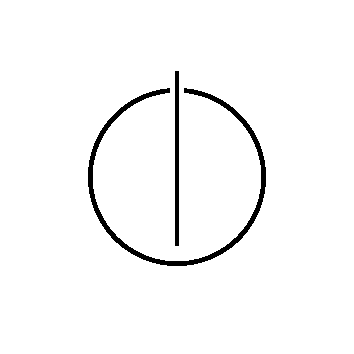
\includegraphics[width=4cm]{styles/informat.png}
  \end{figure}
  
  \end{center}
%	\clearemptydoublepage
%	
%	% The titlepage for the CAMP report document.
% Included by MAIN.TEX


%--------------------------------------------------
% The title page
%--------------------------------------------------

% correct BCOR - undo at the end !!!
\def\bcorcor{0.15cm}
\addtolength{\hoffset}{\bcorcor}

\thispagestyle{empty}

 \vspace{10mm}
\begin{center}
	       \oTUM{4cm}
	   
	   \vspace{5mm}     
	   \huge FAKULT{\"A}T F{\"U}R INFORMATIK\\ 
	   \vspace{0.5cm}
	 \large DER TECHNISCHEN UNIVERSIT{\"A}T M{\"U}NCHEN\\
        
	\end{center}
		

\vspace{10mm}
\begin{center}

   {\Large \doctype}

  \vspace{10mm}
  
  {\LARGE \title}\\
  
  
  \vspace{10mm}
  
  
  {\LARGE  \titleGer}\\
  
  
  \vspace{10mm}

    %\hfill
    \begin{tabular}{ll}
	   \Large Author:     & \Large \author \\[2mm]
	   \Large Supervisor:    & \Large Prof. Dr. Bukhard Rost \\[2mm]				
	   \Large Advisor:	& \Large Mr. Juan Miguel Cejuela P{\'e}rez\\[2mm]
	   \Large Date:       & \Large December 12, 2014
	 \end{tabular}
	 
	 \vspace{5mm}
	 
	 \begin{figure}[h!]
  \centering
   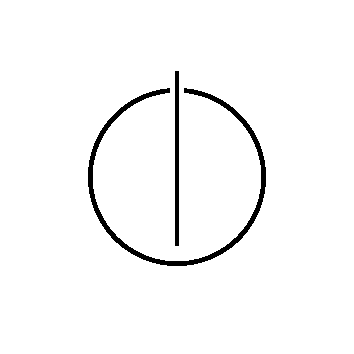
\includegraphics[width=4cm]{styles/informat.png}
  \end{figure}
   

\end{center}

% undo BCOR correction
\addtolength{\hoffset}{\bcorcor}
	
	
%	\input{components/cover_maschmeyer}
	\clearemptydoublepage
	
	% The titlepage for the CAMP report document.
% Included by MAIN.TEX


%--------------------------------------------------
% The title page
%--------------------------------------------------

% correct BCOR - undo at the end !!!
\def\bcorcor{0.15cm}
\addtolength{\hoffset}{\bcorcor}

\thispagestyle{empty}

 \vspace{10mm}
\begin{center}
	       \oTUM{4cm}
	   
	   \vspace{5mm}     
	   \huge FAKULT{\"A}T F{\"U}R INFORMATIK\\ 
	   \vspace{0.5cm}
	 \large DER TECHNISCHEN UNIVERSIT{\"A}T M{\"U}NCHEN\\
        
	\end{center}
		

\vspace{10mm}
\begin{center}

   {\Large \doctype}

  \vspace{10mm}
  
  {\LARGE \title}\\
  
  
  \vspace{10mm}
  
  
  {\LARGE  \titleGer}\\
  
  
  \vspace{10mm}

    %\hfill
    \begin{tabular}{ll}
	   \Large Author:     & \Large \author \\[2mm]
	   \Large Supervisor:    & \Large Prof. Dr. Bukhard Rost \\[2mm]				
	   \Large Advisor:	& \Large Mr. Juan Miguel Cejuela P{\'e}rez\\[2mm]
	   \Large Date:       & \Large December 12, 2014
	 \end{tabular}
	 
	 \vspace{5mm}
	 
	 \begin{figure}[h!]
  \centering
   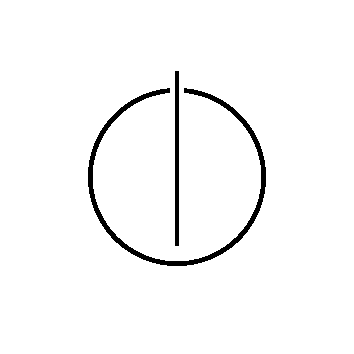
\includegraphics[width=4cm]{styles/informat.png}
  \end{figure}
   

\end{center}

% undo BCOR correction
\addtolength{\hoffset}{\bcorcor}
	
	
	\clearemptydoublepage


\thispagestyle{empty}
\selectlanguage{german}
	\vspace*{0.7\textheight}
	\noindent
	I assure the single handed composition of this master's thesis only supported by declared resources.
	\\
	\\
	Ich versichere, dass ich diese Masterarbeit selbst{\"a}ndig verfasst und nur 
	die angegebenen \\Quellen und Hilfsmittel verwendet habe.
	
	\vspace{15mm}
	\noindent
	M{\"u}nchen, den \today \hspace{5cm} \author
\selectlanguage{english}
\newpage
	


	
   
	\mainmatter
		% Abstract for the TUM report document
% Included by MAIN.TEX


\clearemptydoublepage
\phantomsection
\addcontentsline{toc}{chapter}{Abstract}





\vspace*{2cm}
\begin{center}
{\Large \bf Abstract}
\end{center}
\vspace{1cm}
This thesis introduces a new coreference resolution system for biomedical texts. This system identifies and links expressions (definite nouns and pronouns), which refer to proteins. I focus on improving the current state-of-the-art in coreference resolution for abstracts and, a novel aspect, apply the system on full-text articles. The system uses syntactic rules to resolve pronouns, and  a string-matching method  and domain knowledge together with the C5.0 classifier to resolve definite noun anaphoras. \\
  Furthermore, the lack of a corpus with full text articles negatively impacts  this area of research. To overcome this problem, I annotated 10 full-text documents, containing: proteins, coreference, and anaphora-antecedent relations.
  During this thesis I collected statistics from the existing BioNLP corpus of abstracts and reviewed current coreference resolution methods in other non-biomedical corpora.
  The system achieves 73\% precision and 75\% recall in the BioNLP development set and 72\% precision and 57\% recall in the test set. On my annotated full-text articles, the precision is 75\% and recall is 65\%.

% Juanmi: it makes no sense to highlight the creation of the full text corpus (btw 8 or 10 documents?) here in the abstract and then on the actual thesis body don't even dedicate to this aspect a small section. That is, either you remove this comment from the abstract, or rather create a section in the body (better)

% Juanmi: highlight that your performance is better than the current state of the art on abstracts.
	
		\clearemptydoublepage
\phantomsection
\addcontentsline{toc}{chapter}{Acknowledgements}	


%\chapter*{Acknowledgements}

\vspace*{2cm}

\begin{center}
{\Large \bf Acknowledgments}
\end{center}

\vspace{1cm}




I would first like to thank my supervisor prof Burkhard Rost for his support and opportunity to do my master's thesis in his group.

 A great thanks goes for my advisor Juan Miguel Cejuela for his advises during thesis. His advises in research, organization, communication and bioinformatic were  evident in every moment during the period of thesis.  

I want  to extend my gratitude to the whole Rostlab group for creating a great environment to work in. Special thanks go to Tim Karl, who responded in every my request. 


	
		\tableofcontents
	
	
		% ---------------------------------------------------------------------------
		%
		%Introduction and Background Theory
		%
		% ---------------------------------------------------------------------------
		\part[Introduction and Theory]{Introduction and Theory}
		\label{part:introAndBackgroundTheory}
		\chapter{Introduction}
\label{chapter:Introduction}
\section{Coreference resolution}

Coreference resolution is the process of determining whether two or more expressions in natural language refer to same entity in the real world [4]. Coreference resolution is an important and challenging task of natural language processing (NLP) [1,5]. It is believed to be useful in question answering, information extraction, relationship extraction and document summarization among others. \vspace{5mm}
  
\emph{Example (1):}
\begin{changemargin}{10mm}{10mm} 
   \emph{ M-CSF treatment was also associated with a rapid induction of \textbf{the jun-B gene}, although expression of \textbf{this gene} was prolonged compared to that of c-jun.}          
   \vspace{5mm} 
\end{changemargin} 

In example (1), \emph{\textbf{ "the jun-B gene"}} and \emph{ \textbf{"this gene"}} refer to same entity in the real world. Therefore, we can say that these two expressions corefer. Another characteristic of these two expressions is that the second expression is semantically dependent on the first.

This dependency of corefering expressions leads to a new linguistic phenomenon called anaphora. Linguists have given various different definitions for these two linguistic terms, which leads to a conflusion between coreference and anaphora. Sometimes researchers do not distinguish these two terms and say that they are synonyms [2]. For clarification, in the following paragraphs I will give the definitions of anaphora and coreference that we will use throughout the thesis.
  
Anaphora (anaphoric expression) is the linguistic phenomenon of pointing back to a previously mentioned expression in the text. The expression mentioned in the text which an anaphora points to is called the antecedent. Anaphora resolution is the process of finding the antecedent of an anaphoric expression [73]. In other words, it means finding pairs of anaphoras and antecedents. As illustration, in example (1) \emph{\textbf{ "the jun-B gene"}} is an anaphoric expression (anaphora) because it refers back to its antecedent, \emph{ \textbf{"this gene"}}. 

If the antecedent and anaphora refer to a same entity in the real world they are coreferential [73].

Gasperin defines anaphora as a directed relation between two linguistic expressions in the text, where the reader, in order to interpret the second expression, is referred back to the first one. In Figure 1.1 we can see the intersection and difference between coreference and anaphora. The intersection of these two terms is coreferent anaphora. Thus, a coreferent anaphora is when the anaphoric expression is dependent from the antecedent and they refer to same entity [49].

Associative anaphora is a relation between two expressions where the anaphora's interpretation depends on the antecedent, but nevertheless, they do not semantically refer to a same entity. In example 2, \emph{"the door"} is an associative anaphora and its antecedent is \emph{"the room"}, because to interpret the expression\emph{"the door"} we need to refer back to the expression \emph{"the room"}.\\

\emph{Example (2):}
\begin{changemargin}{10mm}{10mm} 
   \emph{  The student entered in \textbf{the room}. He did not close \textbf{ the door}.}
   \vspace{5mm} 
\end{changemargin}  
\begin{figure}[ht]
   \begin{center}
	  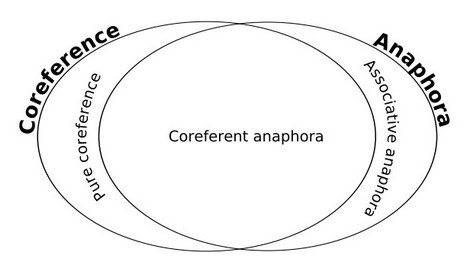
\includegraphics[scale=1.]{corefVsAnaphora.jpg} 
 	  \caption[Difference between anaphora and coreference]{Difference between anaphora and coreference [49]}
	  \label{Figure 1}
   \end{center}
\end{figure}

Kees van Deemter and Kibble [24] define coreference relation of two expressions as the logical equivalence relation where both expressions \emph{"refer to the same entity"}.
 
Mathematically, defining Referent$(\alpha_1)$ as the\emph{"the entity referred to by $\alpha_1$"}, a coreference relation for expressions $\alpha_1$ and $\alpha_2$ holds if and only if 
\begin{center}
  Referent $(\alpha_1)$ = Referent $(\alpha_2)$
\end{center}
 
Hence, coreference is an equivalence relation (reflexive, symmetric and transitive relations). From symmetric relation, the conclusion is that $\alpha_1$ and $\alpha_2$ are semantically independent. Furthermore, the authors [24] define anaphoric relation of two expressions $\alpha_1$ (antecedent) and $\alpha_2$ (anaphora), if and only if $\alpha_2$ depends on $\alpha_1$ for its interpretation. 
 
Summarizing, anaphora resolution is the task of finding mentions (anaphoras) that are dependent in their interpretation on a second expression (their antecedent). On the other hand, coreference resolution can be seen as a clustering task, where we have to find all mentions in the text that refer to same entity.

\section{Coreference resolution in Biomedical literature}

In biomedical literature, there exists just one corpus that deals with coreference resolution. This corpus was published by the BioNLP group. In it, the community defined the task named Protein Coreference Resolution. I will describe in the following sections the detailed specification of this task.

\subsection{Data description}

The BioNLP corpus consists of 1210 annotated abstracts. The corpus is divided into 3 subsets: 800 abstracts in the training set, 150 in the development set, and 250 in the test set. Each document is annotated with proteins, anaphoric expressions and their references. For each abstract, three files exist:
\begin{itemize}
  \item A text file, which contains the content of the abstract.
  \item A protein annotation file, which contains the annotated proteins.
  \item A relation file, which contains the coreference relation.
\end{itemize}

\newpage
\begin{figure}[ht]
   \begin{center}
	  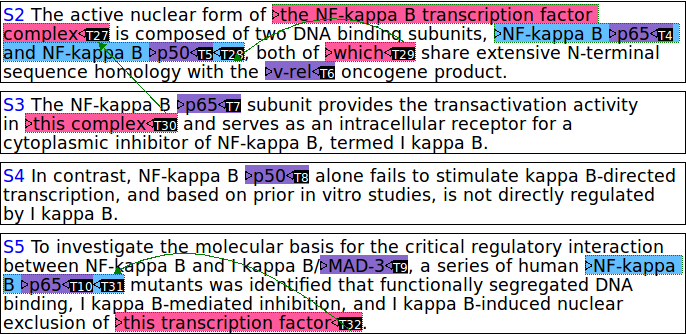
\includegraphics[scale=0.6]{bioNLP.jpg} 
      \caption[Example of file annotation]{Example of file annotation\footnotemark}
	  \label{Figure 2}
   \end{center}
\end{figure}
\footnotetext{Figure taken from [63]}

I will clarify the content of the protein annotation and coreference relation files by examples. In Figure 1 .2annotations T4-10, marked with purple color, are protein annotations. Every protein name mentioned in the text is annotated. Each annotation consist of its id, offsets (begin span and end span) and its string content, and this information is inserted in the protein annotation file as in Example (3).\\

\emph{Example (3):}
{\fontfamily{qcr}\selectfont
	\begin{tabbing}
		\hspace{3cm} T4	\hspace{5mm}\=  Protein 275 278	\hspace{5mm} \= p65\\
		\hspace{3cm} T5 \> Protein 294 297 \> p50\\
		\hspace{3cm} T6	\> Protein 367 372 \> v-rel\\
		\hspace{3cm} T7	\> Protein 406 409 \> p65\\
		\hspace{3cm} T8	\> Protein 597 600 \> p50\\
		\hspace{3cm} T9	\> Protein 843 848 \> MAD-3\\
		\hspace{3cm} T10 \> Protein 879 882 \> p65\\
	\end{tabbing}
}
\vspace{5mm} 

\emph{In Example (3), the first line indicates that in the text there is a protein reference \textbf{"p65"} that begins at 275th character and its content ends before 278th character. This annotation is indexed by the id, "T4" [1].}

The coreference relation file contains three types of annotations: anaphoric annotations, their antecedent, and coreference relations. In Example (4), annotations T27-32 are of the first and second type and the R1-R3 describe coreference relation of expressions. Most of the anaphoric expressions are: pronouns (relative, personal, possessive, reflexive) and definite nouns (e.g. this protein).\\

\emph{Example (4)\footnotemark :}
{\fontfamily{qcr}\selectfont
	\begin{tabbing}
		{\small T27 \= Exp 179 222\hspace{3mm} \= the NF-kappa B TF compl 215 222 compl} \\
		{\small T28 \> Exp 264 297 \> NF-kappa B p65 and NF-kappa B p50}\\
		T29 \> Exp 307 312 \> which\\
		T30 \> Exp 459 471 \> this complex \hspace{2mm}   464 471 complex \\
		T31 \> Exp 868 882 \> NF-kappa B p65\\
		T32 \> Exp 1022 1047 \> this TF   1027 1047  trans. factor\\
		R1  \hspace{5mm} \=  Coref Anaphora:T29 Antecedent:T28  \hspace{5mm}  \= [T5, T4]\\
		R2 \>  Coref Anaphora:T30 Antecedent:T27\\
		R3 \>  Coref Anaphora:T32 Antecedent:T31  \>  [T10]\\
	\end{tabbing}
}
\footnotetext{Transcription factor is shorten in TF and complex in compl because of limited line space}
\vspace{5mm} 

\emph{In Example (4), the first line indicates that in the offset 179-222 of the abstract there is a protein mention "the NF-kappa B transcription factor complex". Its minimal , which still carries its meaning, is "complex" (215-222), and this annotation has the index "T27". In this way, every annotation (a protein mention or an expression that refers to a protein) is described in the coreference relation file.}

\emph{The last line describes the coreference relation between mentions T32 and T31. Also, we can see that mention T32 is an anaphora and refers to T31, which in its string contains a protein name T10 (p65). So, here we see that we have two types of coreference relations. The first type of relation is between two corefering mentions, like T32 with T31, and the second type of relation is between a mention and a protein name (T32 with T10).}

\subsection{Task description and evaluation}

For both types of coreference relations the BioNLP community (mentioned in the previous section) defined a sub-task. First relation type is named surface coreference resolution and the latter is named protein coreference resolution.

For both tasks, the resolver receives a text and a protein annotation file, and as output should return all protein mentions with their offsets and coreference relations between mentions. The result should be a file similar to Example (3), with all detected protein mentions and relations. 

\subsection{Evaluation Measures}

In this section, I will define the Protein Coreference Resolution task(in abstracts and full text) mathematically and its evaluation measures. The task($f$) of protein coreference resolution, which is defined by the BioNLP community, I define formally in the following way:" given a text (abstract) $T$ with annotated protein names $P$, the system should return ordered couples $(x, y)$ where $y$  is the antecedent of $x$".\\
\begin{center}
  $f(X,P)=\{(x_i,y_i) |i=1..n \And Antecedent(y_i)=x_i \And y_i= protein$  $name\}$ \\
  $X-string$ \\
\end{center}

$P$ is a set of ordered set defined in the following way:\\
\begin{center}
    $P= \{(start_j, end_j, protein_j)| j=1..n \And start_j< end_j \And |protein_j|= end_j-start_j\}$\\
\end{center}
 
The system that I built produce three types of anaphora-antecedent links(pairs):

\begin{itemize}
  \item correct response links
  \item missing links
  \item spurious response links.
\end{itemize}
From these three types of links we can derive:
\begin{itemize}	
 \item $true$ $positive$ $(tp)$ - number of  correct anaphora-antecedent links - links that the system correctly predicted\\
 \item $true$ $negative$ $(tn)$ - number of missing anaphora-antecedent links - links that the system did not find\\
 \item $false$ $positive$ $(fp)$ - number of spurious anaphora-antecedent links - links that the system predicted wrong \\
\end{itemize}
To measure the accuracy of the system we use the traditional  precision, recall and F-score  measurement which are defined in the following way\\
\hspace{2cm}  Precision: \hspace{1cm}\\
\hspace{4cm}\[ \scalebox{1.2} {$P =\frac{tp}{tp+fp}$}\] \\
\hspace{2cm} Recall: \\
\hspace{4cm} \[ \scalebox{1.2} {$R=\frac{tp}{tp+tn}$}\] \\
F-score is taken as equally weighted harmonic mean of precision and recall:\\
\[ \scalebox{1.2} {$F(\beta)=(1+\beta^2)\cdot \frac{P\cdot R}{\beta^2P+R}$}\] \\
 and for $\beta=1$ \\
\[ \scalebox{1.2} {$F(1)=2\cdot \frac{P \cdot R}{P+R}$}\]\\
\subsection{Evaluation measures in BioNLP Protein coreference resolution}

In the surface coreference mode, the resolvers should find anaphoric protein expressions and their antecedents, regardless of whether antecedent actually embed protein names or not. 
The protein coreference mode evaluates the performance of finding anaphoric protein references, which their antecedent contains a protein name. 
My main focus in this thesis was to build a system which achieves high accuracy in protein coreference mode. Thus, I will describe the scoring principle of protein coreference mode using an example.

From example (4) we take relation \emph{"R1 Coref Anaphora:T29 Antecedent:T28 [T5, T4]"}. Antecedent T28 contains two protein names \emph{p50} and \emph{p65}. So, in the protein coreference mode, we check whether (T29, T5) and (T29,T4) are predicted or not. For each of these pairs, if the system predicted, it gets 1 point. The whole R1 has two points. If the system finds just (T29,T5), it gets 1 point. Wrong predicted pairs decrease the system's precision. 

\subsection{Importance of coreference resolution}

Why is coreference task important in biomedical domain?

Coreference resolution is believed to be useful for improved event and relationship extraction [2]. Until now we do not have concrete results to prove that the coreference resolution improves the Information extraction in biomedical domain, because the protein coreference task did not have enough good results and the motivation of this thesis was to build a high accurate coreference resolution system.
 
In other domains, anaphora resolution improves results in different information extraction and machine translation tasks (see section 2), but still the improvements are not as expected because of the accuracy of current anaphora resolution systems[9,10,11,12].
 
Anaphora resolution is not a high-accuracy task for information extraction (IE) systems but properly resolving some kinds of coreference is usually difficult even for humans annotators, who achieved about 80 percent [8].



		\chapter{Natural Language Processing}
\label{chapter:Natural Language Processing}
\section{Natural Language Processing: Concepts}

Natural language processing (NLP) is a research area for the analysis, understanding, and generation of written and spoken natural language [13,14]. Coreference resolution is a task of NLP.

I had to use different NLP tools to analyse the text. These tools helped  the coreference resolution system to understand the text and to find coreference links in it. The quality and robustness of these tools directly influence the performance of my system. To build a high performance coreference resolution system for biomedical domain, I used NLP tools that are built and trained in biomedical data sets.

In the following sections I will explain some NLP tasks that are used to build the used tools and the coreference resolution system. Additionally, I will explain terms that I will use in the next chapters. In the beginning, I will describe the tasks, which help coreference resolution to increase its accuracy. In the latter sections, I will describe the NLP tasks that coreference resolution (is believed) to help.

\subsection{NLP tasks that help coreference resolution}

\emph{ \textbf{ Sentence segmentation (sentence splitting)}} is the process of dividing a text into sentences. This process usually receives a text (paragraph or article) as input and returns the text divided into sentences as output.
In the English language, this process is rather simple because typically sentences end with a full stop. Nevertheless, the full stop can be ambiguous when we use it in numbers as decimal separator (9.85), in websites (www.in.tum.de), and in abbreviations (M.Sc.). In the biomedical domain, these ambiguous phenomenon occurrences are evident.
Despite these occurrences, the sentence splitter GeniaSS [55] is an accurate sentence splitter system, which is trained in biomedical data. GeniaSS achieves an F-score of 99.7 on 200 unseen GENIA abstracts [15].\\

\emph{ \textbf{ Word segmentation}} is the process of dividing a sentence into words. In languages that have a specified word delimiter the word segmentation task is trivial. The English language uses space as word delimiter. There are cases where between  two words does not exist a separator because they are connected by an apostrophe. This construction of two words (without separator) is handled accurately by word segmentation systems. In the English language, the accuracy of the best systems is 99.4-100\%. Languages that do not use a word separator word segmentation is not an easy task. Despite this, languages that do not have word delimiters (e.g., Chinese and Japanese) the accuracy of word separators is in the range of 92-98\%.\\

\emph{ \textbf{Tokenization}} is the process where a text is divided into small individual units. Each of these units is meaningful and it is called token. Most of the tokens coincide with words of the text in which the tokenization is being performed [8]. In tokenization we define a scheme how to divide the text.\\

\emph{ \textbf{Part of speech (POS) tagging}} is the process of assigning the part of speech class to a token/word. The English language has eight part of speech classes, namely: nouns, verbs, adjectives, adverbs, pronouns, prepositions, interjections and conjunctions.

Each language has its part of speech classes. For example in the Albanian language there are 11 part of speech tags.\\

\emph{ \textbf{Parsing(deep parsing)}} is the process of representing the sentence's syntactic structure in a tree, where the leaves of the tree are tokens. This process provides a detailed structure of the sentence (the tree). Deep parsing is one of the most important tasks in text and speech processing, because it gives the detailed structure of the sentence, relationship between words/tokens and their role in the sentence.\\

\emph{ \textbf{Shallow parsing (or light parsing or chunking)}} is a similar task to deep parsing, but it does not give a detailed structure of the sentence. This process just identifies the tokens and assigns part of speech class to each chunk.\\

\emph{ \textbf{Parsing direction}} refers to the direction in which a sentence is parsed. Parsing can be performed in two directions: from left to right (forward direction), and from right to left (backward direction). The direction of parsing a sentence has an important role in the precision and the speed of a parser. Note that this is also important considering that different languages are written in different directions.\\

\emph{\textbf{Lemmatization}} is the process of removing the prefixes and/or suffixes of a word/token. The lemmatization process transforms a word to its base (pure) form, which is called lemma. This transformation of the word does not change its meaning. The lemmatization process uses dictionaries to find the lemma of the word and deals with irregular forms of words. For example the words transform, transformed, transforming, transformation are all formed from the lemma \emph{transform}. A similar process to lemmatization is steaming, which finds the root of a word.  Root of the word is the part, which carries the semantic content of it. The stemming process can not handle the irregular forms of the words and do not use dictionaries.\\ % The difference is not well explained, not clear

\begin{figure}[ht]
   \begin{center}
	 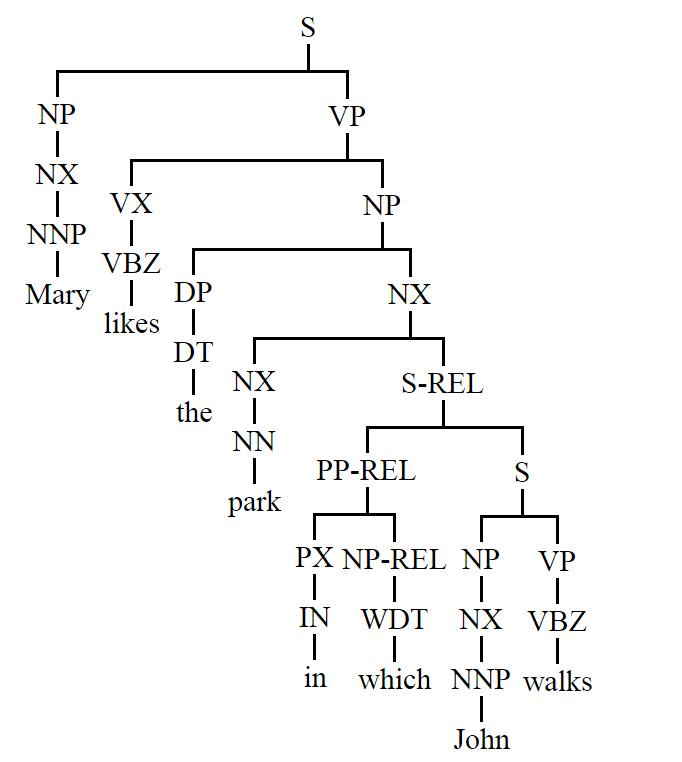
\includegraphics[scale=0.4]{EnjuParser1.png}
 	 \caption[Tree structure of a sentence]{Tree structure of a sentence}
	 \label{Figure 3}
   \end{center}
\end{figure}

\emph{\textbf{Spelling correction}} is the process in which misspelled words are corrected. Spelling correction systems are called spell checkers. Modern spell checkers (like Google's) not only correct individual misspelled words of a sentence but also have a holistic approach and try to correct the words such that the sentence as a whole becomes semantically correct. To achieve better results, spelling correctors use dictionaries and \emph{n-grams}.\\

\emph{\textbf{Word-sense disambiguation}} is the process of determining the meaning of a word. In the real world, it can happen that a word can have two or more meanings. For example, the word desert has two different meanings,a territory with sand and a dish. These "two" words, which have the same spelling, but different meanings are called homonyms.

Another linguistic phenomenon, polysemy, is when two or more words have the same spelling, and distinct and related meanings. The word "mouth" can be considered as polysemes because it can mean orifice on a face or opening of a cave or river.

Another case of word sense disambiguation are capitonyms. This is when a word has one meaning when it is capitalized, and different meaning when is not capitalized. For example the words "polish" and "Polish", which mean to make shiny and a person from Poland, respectively. \\

\emph{\textbf{Abbreviation expansion}}is the process of resolving the full expansion of an abbreviation. A system that deals with abbreviation expansions saves every pair of abbreviation and its full expansion; and then in every new occurrence of an abbreviation it refers back to the saved abbreviation and its expansion. Abbreviations in biomedical text appear often. \\

\subsection{NLP tasks that coreference resolution helps}

\emph {\textbf{ Name entity recognition (NER)}} is the process in information retrieval that identifies and classifies mentions in a text that corresponds to a target group (entities) in which we are interested in. For example, in the biomedical domain we are interested in identifying proteins, genes, mutation and viruses. \\

\emph{\textbf{Relationship extraction}} is the process of identifying relations (in a text) between predefined entities. In biomedical information extraction community, the motivation of building an efficient coreference resolution system is that the community believe that coreference resolution improves accuracy of relationship extraction of biomedical entities. \\

\emph{\textbf{Machine translation}} is the process of translating a text or a speech from one language to another. These software products that translate a text from one language to another use different statistics and syntactic rules to translate one text to another. Modern machine translation systems use probabilistic models and rules to produce better translation. \\

\emph{\textbf{Question answering and natural language interfaces}} are tasks that allow humans to communicate with a computer bot. This communication is done in question and answer format. In this situation, humans ask a computer bot and the computer bot answers the humans by voice or text. In conversion (text or voice), people use pronouns and anaphoric expressions and the computer bot should resolve these anaphoric expressions. For this purpose, coreference and anaphora resolution are important components of question answering and natural language interfaces.\\

\emph{\textbf{Document summarization}}  is the process of identifying the essence of the text. This process takes a large text, as input, and return a grammatically and semantically correct smaller text, which contains the essence and the main content of the inputted text. \\

\section{Syntax}

Syntax(etymology: a Greek word syntaxis=syn [together] + taxis [arrangement]) is a discipline of linguistic, which studies the rules and patterns of ordering and connecting words in the sentence, such that the created structure of the sentence is grammatically correct.

\subsection{Words}

Words and grammatical rules are the fundamental elements to creating a grammatically correct sentence. We should be aware, that if a sentence is grammatically correct, it does not mean that it has a meaning.

These smallest units, words, are classified in different classes based on a characteristics and their function in the sentence. The main characteristic of every word is its part of speech class. Part of speech classes are divided in two subclasses: opened and closed. In the open class are: nouns (N), adjectives (ADJ), adverbs (ADV) and verbs (V). Open part of speech classes have a meaning and every open part of speech class can be extended, thus in these  classes can enter new words. In the closed set are: determiners (DET), prepositions (PREP), conjunctions (CONJ) and pronouns (PR). These part of speech classes are closed and their set of words is a fixed set.

\subsection{Phrases}

Phrase is a sequence of words, that inherits the characteristics of one of the words, which is called the head word. The phrase has a part of speech class and it inherits its part of speech class from its head word. From this characteristic, logic follows that a phrase can contain phrases and it has a recursive structure.

Other words of the phrase modify, distinguish the head object from other similar objects and give more information about the head object. These words are called modifiers.

Based on the head word, we have different type of phrases; for example noun phrases (NP) and verb phrases (VP).

\newpage
\begin{figure}[h]
   \begin{center}
	  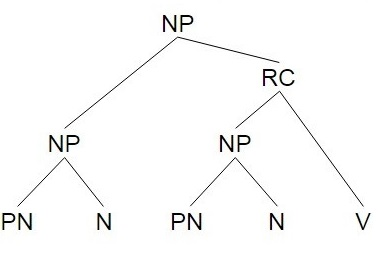
\includegraphics[scale=0.7]{nounPhraseREcursive.jpg}
 	  \caption[Recursive structure of a phrase]{Recursive structure of a phrase}
	  \label{Figure 4}
    \end{center}
\end{figure}

Phrases that their head word is a noun are called noun phrases. Usually singular noun phrases start with a singular determiner (a, an, the, this, any) or start with a proper or a common noun. Plural noun phrases start with a plural determiner (these, those, some..) or start with a plural noun. Pronouns (it, he, they, itself...) are also considered noun phrases.\\

\emph{Example (5):}
\begin{changemargin}{10mm}{10mm}
   \emph{Some rules for creating noun phrases:}
   \begin{itemize}
  	    \item \emph{\itab{ NP $\rightarrow$ N} \tab {student}}
  	    \item \emph{\itab{ NP $\rightarrow$ DET N} \tab {the student}}
  		\item \emph{\itab{ NP $\rightarrow$ DET ADJ N } \tab {the intelligent student}}
  		\item \emph{\itab{ NP $\rightarrow$ ADJ N } \tab {intelligent student}}
  		\item \emph{\itab{ NP $\rightarrow$ NP CONJ NP } \tab {a student and a professor}}
  		\item \emph{\itab{ NP $\rightarrow$ N PP } \tab {student at library}}
   \end{itemize}
\end{changemargin}
\vspace{4mm}

Phrases that their head word is a verb are called verb phrases. Verb phrases consist of a verb and are followed by a noun phrase and/or prepositional phrase. \\

\emph{Example (6):}
\begin{changemargin}{10mm}{10mm}
   \emph{  Some rules for creating verb phrases:}
    \begin{itemize}
  	    \item \emph{\itab{ VP $\rightarrow$ V} \tab {learn}}
  		\item \emph{\itab{ VP $\rightarrow$ V NP} \tab {learn history}}
  		\item \emph{\itab{ VP $\rightarrow$ V PP NP } \tab {learn at home}}
	\end{itemize}
\end{changemargin}

\vspace{4mm}

Prepositional phrases, another type of phrases in English language, consist of a preposition and a noun phrase. Prepositional phrases are used to define more specifically a noun phrase. Thus, we can say that their role is similar to adverbs and adjectives.

\subsection{Clauses}

Clauses are linguistic units that contain a noun phrase and a verb phrase. The clauses are divided into two types: dependent and independent.

\subsection{Independent clause}

An independent clause is a grammatically correct group of words that contains a noun phrase that acts as the subject of clause and a verb phrase.

The independent clause has a meaning, expresses a thought and can form alone a sentence. If a sentence has more than one clause then at least one of the clauses is independent. One of the independent clauses is main and it carries the subject and meaning of the sentence, and is called main clause.

If the sentence has two or more independent clauses they are called coordinated clauses and they are connected with a coordinating conjunction. The coordinated conjunctions are: and, but, for, nor, or, so, and yet.

Alternatively instead of a conjunction, we use a comma to connect two coordinated clauses.

\subsection{Dependent clauses}

A dependent clause is a grammatically correct group of words that contains a noun phrase (NP) and a verb phrase (VP), and it has not semantic meaning. Dependent clauses are also called subordinate clauses, because their role in the sentence is secondary. This means that if a sentence has a dependent clause, then there exist another clause that is main and independent, and the subordinate clause is dependent on the main clause. The role of subordinate clauses in the sentence is similar to adverb or adjective; they are used to describe a property, cause or a consequence of an object or a noun phrase of the main clause. Usually, the subordinate clauses are connected with the main clause or another subordinate clause with an subordinate conjunction or relative conjunction. Examples of relative conjunctions include: who, whom, that, which, what and whose; and examples of subordinate conjunctions include: although, because, if, unless, as, until, even though, even, before and when.

\subsection{Sentences}

We use sentences to express our needs, emotions, ideas, thoughts and curiosity among others. Depending what we express, we use 4 types of sentences:
\begin{itemize}
	\item declarative sentences, to make statements (.)
	\item interrogative sentences, to ask questions (?)
	\item imperative sentences, to give commands (.or !)
	\item exclamatory sentences, to express strong feelings (!)
\end{itemize}

In the biomedical articles sentences are in declarative form. Thus, I will describe the structure of the declarative sentences. In the text below, I will use the terms declarative sentence and sentence interchangeably.

A declarative sentence has at least one independent clause, and express a thought. It contains a subject (what or whom the sentence is about) and a verb (the action that the subject takes). There are cases that a sentence expresses a thought and do not contain either verb or subject. This type of sentence is called ellipsis. Ellipsis are common in dialogue. In ellipses, the speaker (writer) assumes a prior knowledge and common sense knowledge from the co-speaker (co-writer).

English language has a defined structure of the sentence and it is an ordered Subject-Verb-Object structure.This structure helps to know the position of the main parts of the sentence.

Another classification of sentences is based on the number and type of clauses that compose the sentences. These types are: simple, compound, complex and compound-complex sentences.

\emph{\textbf{Simple sentence}} consist just from one independent clause.\\

\emph{Example (7):}
\begin{changemargin}{10mm}{10mm}
   \emph{Proteins are assembled from amino acids.}
\end{changemargin}
\vspace{3mm}

\emph{\textbf{Compound sentences}} consists of two or more coordinated clauses connected with coordinated conjunction.\\

\emph{Example (8):}
\begin{changemargin}{10mm}{10mm}
  \emph{Bioinformatics is a science and bioinformaticians research bioinformatics.}
\end{changemargin}
\vspace{3mm}
\newpage
\emph{\textbf{Complex sentences}} consists of one independent clause and one or more subordinate clause.\\

\emph{Example (9):}
\begin{changemargin}{10mm}{10mm}
  \emph{Natural language processing is important because it helps computers to understand human language.}
\end{changemargin}
\vspace{3mm}

\emph{\textbf{Compound-complex sentences}} consists of three or more clauses, which two or more are coordinated clauses and one or more subordinate clauses.\\

\emph{Example (10):}
\begin{changemargin}{10mm}{10mm}
  \emph{Bioinformatics is a science and bioinformaticians research bioinformatics, because they want to develop mathematical models and software tools to get knowledge from biological data.}
\end{changemargin}
 \vspace{3mm}
As we can see, all these types of sentences have a specific construction. We can see that the subjects of clauses in a sentence are correlated and they tend to have same lemma, are synonyms or coreferential expressions. This construction of the sentences and this correlation between subjects of clauses helps to resolve coreference resolution.

		
		%
		%% ---------------------------------------------------------------------------
		%%
		%% Fully Automated Calibration for Ultrasound
		%%
		%%% ---------------------------------------------------------------------------
		\part[Coreference Resolution]{Coreference Resolution system }
		\label{part:secondP}
		\chapter{Coreference resolution}
\label{chapter:Coreference resolution}
\section{History}

First algorithms for coreference and anaphora resolution date in the '70 of the last century. The first algorithm was published by Hobbs[46,47] in 1976. This algorithm, a pronominal anaphora resolution algorithm, resolved pronouns "he", "she",  "it". Basically, this algorithm was based on syntax rules and heuristics and these rules are:

\begin{itemize}
	\item anaphora and antecedent should corresponds in their gender and number
	\item antecedent of a pronoun is the first NP that can be reached with fewer number of steps
	\item the algorithm uses common sense knowledge (candidate selection)
\end{itemize}

Hobbs tested his algorithm manually in three different text genders (historical, novels and news). He claimed that the naive approach algorithm, without using common sense knowledge, achieves accuracy 88\%, and with common sense knowledge  and with "careful" selection of antecedents achieves accuracy more than 91\%. These accuracies, the algorithm achieved because Hobbs assumed that the parser that build the syntax structure of sentences is a perfect parser.   

In practice, a pronominal anaphora resolution algorithm is difficult to achieve accuracy of around 90\%, because does not exist a perfect parser and does not exist a tool that has a common sense knowledge.

\newpage
\begin{algorithm}[H]
\caption{Hobbs's algorithm}\label{alg:Hobbs}
\begin{algorithmic}[1]
\State Find the $NP$ node immediately dominating the pronoun.
\State Go up the tree to the first $NP$ or $S$ node encountered. Call this node $X$, and call the path used to reach it $p$.
\State Traverse all children of node $X$ to the left of path $p$ in a left-to-right (L-R), breadth first (BF) fashion. Candidate as antecedent any $NP$ node that appear.
\If { node $X$ is the highest node in the sentence} 
	\State traverse the previous sentences in the text in order of recency, the most recent first; each tree is traversed in a L-R, BF manner, and candidate as antecedent any $NP$.
\Else
	\State ($X$ is not the highest node in the sentence) continue to step 9.
\EndIf
\State From $X$, go up to the first $NP$ or $S$ node. Call this new node $X$, and the path $p$.
\If {$X$ is an $NP$ node and if the path $p$ to $X$ did not pass through the $NP$ node that $X$ immediately dominates}
     \State propose $X$ as the antecedent
\EndIf
\State Traverse children of $X$ to the left of $p$ in a L-R, BF manner. Propose any $NP$ node encountered as the antecedent
\If {$X$ is an $S$ node}
    \State traverse children of $X$ to the right of path $p$ in a L-R, BF manner, but do not go below any $NP$ or $S$ node encountered.
    \State Propose any $NP$ node encountered as the antecedent.
\EndIf
\State Go to step 4
\end{algorithmic}
\end{algorithm}

\begin{figure}[h]
	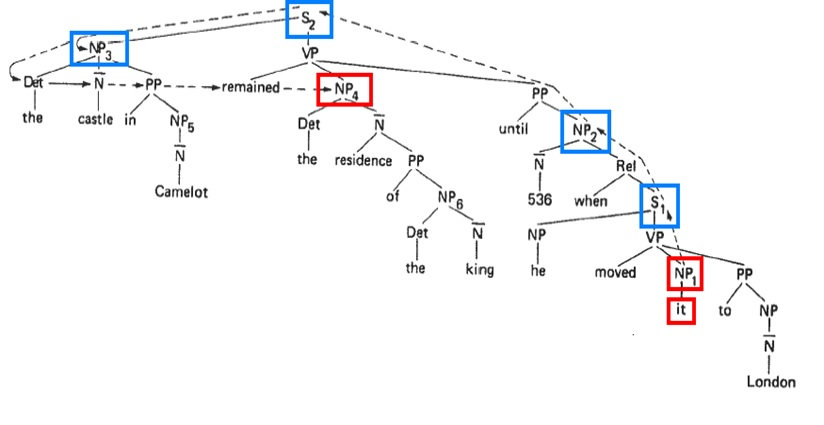
\includegraphics[scale=0.60]{hobbs.jpg} 
 	\caption{Simulation of Hobbs's Algorithm [30,31] }
	\label{Figure 5}
\end{figure}

The trend of building coreference and anaphora resolution algorithms based on common sense knowledge and rules continued in the years 90s (1990-1995). Another characteristic of this period is that did not exist an metric to measure performance of anaphora and coreference resolution systems. Because of this, researchers defined specific evaluation metrics for their algorithms in anaphora and coreference resolution.

In this period scientists Barbara J. Grosz,Aravind K. Joshi, Scott Weinstein [48] publish a theory in coreference resolution. This theory, the centring theory, go further in analysis of coreference and anaphora. To resolve anaphora in their theoretical model they add "relationships among focus of attention, choice of referring expression and perceived coherence of utterances within a discourse segment" [14]. This is the first theoretical model that uses the content of the text in anaphora and coreference resolution.

In mid 90s researchers started to apply coreference and anaphora resolution in information extraction. 

When researchers started to develop coreference resolution systems they needed a standard of coreference resolution algorithms. To have a standard measurement metrics for evaluation of coreference and anaphora resolution algorithms, the computational linguistic community built and annotated a corpus, and defined evaluation measurements, which are the official standards of coreference and anaphora resolution. The corpus and standards were published in the MUC-6 (Message Understanding Conference) conference. The corpus consisted of 60 English language newswire articles. Two years latter the community published a new corpus MUC-7, which was an update of the previous corpus. These two corpuses are most used and famous corpuses. After publishing these two corpuses, different NLP communities published corpuses and evaluation metrics of coreference resolution. Another known corpus, which is used in the computational linguistic is the Automatic Content Extraction (ACE1) corpus. During this period the community was concentrated in building a base theory of coreference resolution. As a result, they defined standards in annotation schemas and the terminology (e.g. markable detection, mention) that is required in coreference and anaphora resolution. 

In the beginning of the year 2000, researchers started using machine learning algorithms in coreference and anaphora resolution. In these methods, they used morphological and structural features: number, gender and part of speech  classes of noun phrases to achieve higher accuracy in the resolution. The researcher Soon et al. (2001) to resolve anaphora generated a set of 12 features. In this set of features Ng and Cardie added 53 other features, including positional, morphological, lexical, syntactic, semantic and even pragmatic features. These methods achieved accuracy around 60-67\%. 

 Meanwhile, the computational linguistic community started to get more interested in coreference and anaphora resolution. As a result, new corpuses in different domains and languages were published. Now, there are annotated and published corpuses in domains: scientific articles, dialogues, news and clinical domain; and in languages:Arabic, Chinese, Dutch, English, French,Italian, Japanese,Spanish and Tibetan language. 

The community realised that a coreference resolution algorithm perform well in one corpus, but achieves poor results in another corpus. This property of algorithms leads to new perception of coreference resolution. Scientists started to develop corpus based coreference and anaphora resolution algorithms. In the last ten years, scientists are using domain specific features and syntactic rules. Depending on the corpus, the results of the best methods achieve accuracy around 70\% in anaphora resolution. [43,65]

\section{Coreference resolution in biomedical domain}

Coreference resolution is believed that helps relationship extraction. This inspired, in 2008, the BioNLP community to build a corpus, with research paper's abstracts, to support other information extraction in biomedical domain. Until now a public corpus with full text articles with protein coreference annotation does not exist.

\section{The state of the art in protein coreference resolution} 

In 2011 was organized a competition in Protein Coreference Resolution. The purpose of the task was to evaluate the effect of coreference resolution in biomedical relationship extraction. In the competition the results in protein coreference resolution were not good enough, the best performing algorithm in protein coreference resolution had an accuracy of 34.1\%. These results were too low to improve relationship extraction tasks in biomedical domain [1]. Organizers of the competition also provided detailed results of best performing algorithms, which are shown in Table 3.1.
\newpage
\begin{table}[h]
  \begin{center}
  \centering
     \begin{tabular}{L{2.0cm} C{2.2cm} C{2.2cm} C{2.2cm} @{}m{0pt}@{}} 
	 	
  		& Precision & Recall & F-score& \\ [1.1ex] 
 		\hline
 		1st place & 73.26 & 22.18 & 34.05& \\ [1.1ex]
 		\hline
 		2nd place & 54.45 & 21.48 & 30.96& \\[1.1ex]
  		\hline
 		3rd place & 63.22 & 19.37 & 29.65& \\ [1.1ex]
  		\hline
	\end{tabular}
  \end{center} 
  \caption{ Results of BioNLP Protein coreference resolution competition [1]}
  \label{table2}
\end{table}

After the competition some research groups were interested to improve the results of protein coreference resolution. One year later, in 2012, were published two papers in protein coreference resolution. In one of the papers authors use semantic classification and rules to resolve protein coreference and achieved an accuracy of 51.3\%. In the second paper authors use an hybrid approach of rules and SVMs and they achieved an accuracy of 60.9\%. This algorithm is the current state of the art in protein coreference resolution.
 
 In the table 3.2, I present results of the best performing algorithms in protein coreference resolution.
\begin{table}[h]
\centering
  \begin{center}
  \centering
 	\begin{tabular}{L{4.2cm} C{2cm} C{2cm} C{2cm}  @{}m{0pt}@{}} 
 		
  		& Precision & Recall & F-score& \\ [1.1ex] 
 		\hline
 		Hybrid approach & 55.6 & 67.2 & 60.9& \\ [1.1ex] 
 		\hline
 		Event miner & 50.4 & 62.7 & 55.9& \\ [1.1ex] 
 		\hline
 		Semantic classification & 52.2 & 50.2 & 51.3& \\ [1.1ex] 
 		\hline
 		Reconcile & 73.3 & 22.2 & 34.1& \\ [1.1ex] 
 		\hline
	\end{tabular}
  \end{center} 
  \caption{Results of the best performing algorithms in Protein coreference resolution}
  \label{table3.2}
\end{table}

A full text corpus with protein coreference annotation does not exist. To evaluate the results of my algorithm in the protein coreference resolution in full text articles I have annotated 8 full text articles, and results of my algorithm in this corpus will be the first  results in the protein coreference resolution in full text.
 
\section{Available tools for biomedical information extraction}

To complete the coreference task, I needed supporting NLP tools for preprocessing and structuring the data set.

For coreference resolution, I used tools that are trained in biomedical domain, because they have better performance than other tools. In the following paragraphs I will describe the tools that I used in my system.

I used the deep parser "ENJU parser", which is trained in biomedical data [50]. Empirically, it is shown that this parser achieves better results in biomedical domain than other parsers [63]. This parser is a Head-driven phrase structure grammar (HPSG) parser. HSPG parsers use semantic and syntactic rules, as well as dictionary to build the tree structure of the sentence [51-57]. The average time of parsing a sentence is 500ms. This parser achieves precision 87.85\% and recall 86.85\% on the Penn Treebank and the average parsing time is 360 ms per sentence [66].

\begin{figure}[h]
  \begin{center}
	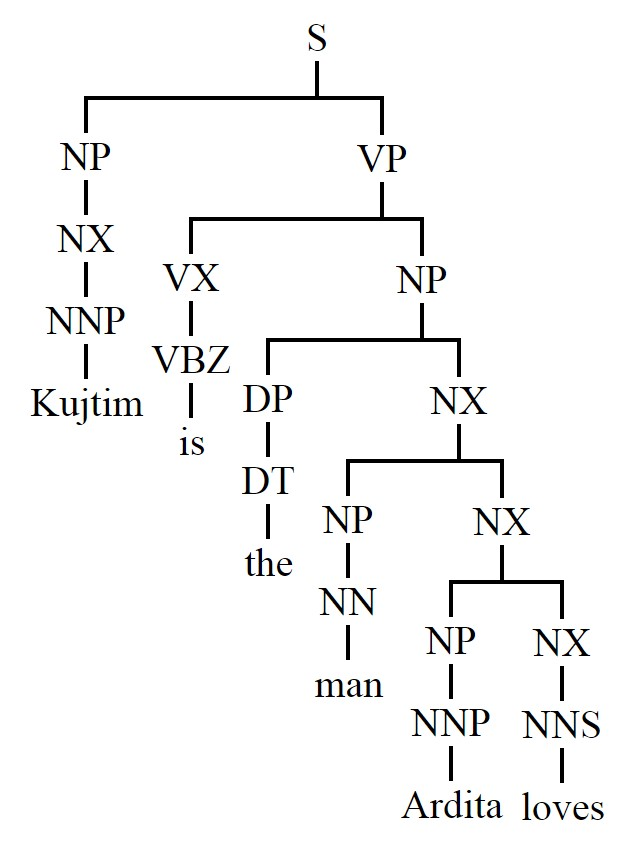
\includegraphics[scale=0.38]{Enju_output.jpg} 
 	\caption[Example output of Enju parser]{Example output of Enju parser [59] }
	\label{Figure 6}
  \end{center}
\end{figure}

An advantage of HPSG parsers is that they give rich linguistic informations. The Enju parser returns the syntactic structure of the sentence in tree. This structure is returned as XML object. In each internal node (not leaf) of the XML object are included these informations: syntactic category (verb, noun phrase preposition,...), extra syntax category (coordinate clause, subordinate clause), and a unique identifier for the node. 

For each token, leaf node of the tree, the parser provides information about the following linguistic characteristics: unique identifier of the token, syntactic category, Penn Treebank-style part of speech tag, base form, and for each token gives its characteristics (words, punctuations). For example for verb, gives following information: the person, the number, the tense, aspect and voice(passive/active). 
\begin{figure}[h]
   \begin{center}
		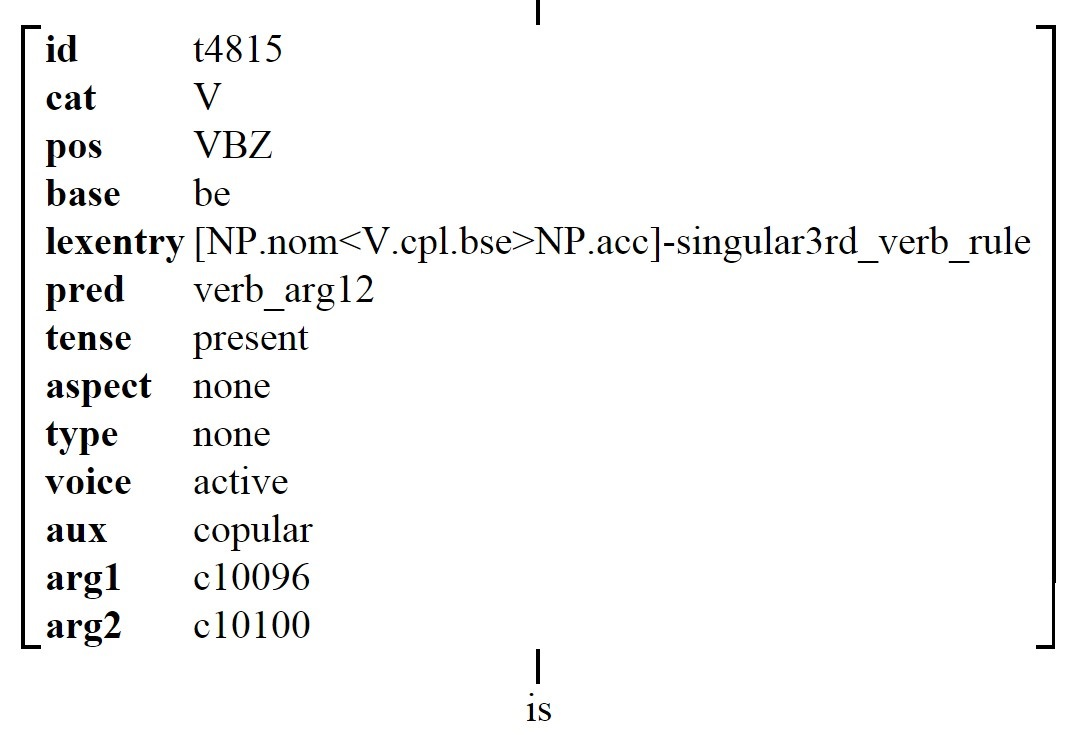
\includegraphics[scale=0.38]{Extended.jpg} 
 		\caption[Information that \emph{Enju parser} gives for the token \emph{is}]{Information that \emph{Enju parser} gives for the token \emph{is}[59]}
		\label{Figure 7}
	\end{center}
\end{figure}
 
Another tool that I used in this thesis is the sentence splitter, GENIA sentence splitter (GeniaSS) [55]. This sentence splitter receives a text (a text file) as input and returns array of sentences (a file where each sentence is written in a specific line). This sentence splitter is trained on supervised learning method using maximum entropy modelling; and it is implemented in C++ [61]. 

GeniaSS is high accurate parser sentence splitter in the Biomedical domain, it achieves an F-score of 99.7\% on 200 unseen GENIA corpus [15].

		\chapter{Coreference resolution using rules and domain-dependent features}
\label{chapter:Coreference resolution using rules and domain-dependent features}
\section{Overview}

In this chapter, I will describe the implementation of a new method in protein coreference resolution. I used corpus based rules to deal with problem of pronominal coreference resolution. 

The corpus consists of  research papers' abstracts, thus, I can assume that the text is written in formal way and authors followed syntax rules. From this hypothesis, I got an idea to  generate syntax rules that model relationship between clauses' subjects  in sentence. 

For definite noun coreference resolution, I use domain dependent features, rules and semantic classification. Also, I realised that the order of the rules influences the accuracy of the system, thus, I defined an order of rules, which I applied on definite noun coreference resolution. This new method effects the result by improving both the recall and precision of the system. 

To build the system, I used the paradigm "divide and conquer". Each type of anaphoric expression is resolved in different way based on its syntax role in the sentence structure. I divided the anaphoric expressions in two main types: pronominal anaphoric expressions and definite noun (phrase) anaphoric expressions. 

Because pronouns can have different role in the sentence, I divided  pronouns into three classes:

\begin{itemize}
	\item relative pronouns: that, which, whom and whose 
	\item personal pronouns: it and they 
	\item possessive pronouns:its and their
\end{itemize}

To extract these rules, I used the training data set of the BioNLP corpus. First, I generated different statistics of the corpus and calculated the distribution of anaphoric expressions, antecedents and coreference links. 

I used the statistics to get knowledge about the corpus and they led me to research following characteristics of the corpus:

\begin{itemize}
	\item the structure of the training data set via mining
	\item patterns 
	\item structure of the language used in the articles
	\item deeper statistics on anaphors, antecedents and their relationship
	\item clauses relationship in the sentence
	\item anaphora's role in the sentence
	\item syntactic rules
	\item window size of the search space
\end{itemize}

\section{Data set}

As I have described in the first chapter, I have used the training set of BioNLP corpus to derive the rules. I have tested the accuracy of the algorithm in the test set and in the corpus of 8 full text documents that I have annotated in a format similar to the BioNLP corpus. I have annotated this corpus of 8 documents on the www.tagtog.net [67,68], which is a web application tool for annotation. I have compared my algorithm with current state of the art algorithms in the development and the test set of BioNLP corpus.

\section{Coreference resolution system architecture}

Coreference resolution systems have a pipeline architecture. My protein coreference resolution system I developed in Java and  published as an open source tool.\footnote{https://github.com/kujta1/CoreferenceResolution}
\newpage
\begin{figure}[t]
	\begin{center}
		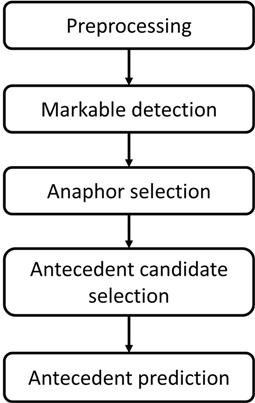
\includegraphics[scale=0.8]{architecture.png} 
 		\caption[Architecture of the coreference resolution system]{ Architecture of the system. As input the system receives two files, the protein annotation file and the text file. The protein annotation file should follow the BioNLP annotation schema. The system after the fifth step, antecedent prediction, will create a file  in which the system will write the coreference links of the inputted text file  [3] }
		\label{Figure 8}
	\end{center}
\end{figure}

The first step of the coreference resolution system is the preprocessing step where the text is dived into sentences. Then, I select all nun phrases the are potential antecedents of an anaphoric expression. In the next step, I select potential antecedent candidates. When  all anaphoric expressions  are selected then for each anaphoric expression I select its potential antecedents. In the final step, I select the most likely antecedent candidate for each anaphoric expression.   
   
In the following sections, I will describe the 5 components of my coreference resolution system. 
  
\begin{table}
   \begin{tabular}{ m{20mm} m{113mm} } 
	\footnotesize{Input (PMID - 7964516)}&\footnotesize{T cell hybridomas respond to activation signals by undergoing apoptotic cell death, and this is likely to represent comparable events related to tolerance induction in immature and mature T cells in vivo. Previous studies using antisense oligonucleotides implicated the c-Myc protein in the phenomenon of activation-induced apoptosis. This role for c-Myc in apoptosis is now confirmed in studies using a dominant negative form of its heterodimeric binding partner, Max, which we show here inhibits activation-induced apoptosis.}\\
	\hline
	\footnotesize{Preprocessing of sentence S3}&\footnotesize{S1: T cell hybridomas respond to activation signals by undergoing apoptotic cell death, and this is likely to represent comparable events related to tolerance induction in immature and mature T cells in vivo. S2: Previous studies using antisense oligonucleotides implicated the c-Myc protein in the phenomenon of activation-induced apoptosis. S3: This role] for c-Myc in apoptosis is now confirmed in studies using a dominant negative form of its heterodimeric binding partner, Max, which we show here inhibits activation-induced apoptosis.}\\
	\hline
	\footnotesize{Markable detection} &\footnotesize{S1: \textit{[T cell hybridomas]} respond to \textit{[activation signals]} by undergoing \textit{[apoptotic cell death]}, and this is likely to represent\textit{ [comparable events related to tolerance induction]} in \textit{[immature and mature T cells [in vivo]]}. S2: [Previous studies using\textit{ [antisense oligonucleotides]}] implicated\textit{ [the c-Myc protein]} in \textit{[the phenomenon of [activation-induced apoptosis]]}. S3: \textit{[This role for [c-Myc] in [apoptosis]]} is now confirmed in \textit{[studies]} using a \textit{[dominant negative form of [[its] heterodimeric binding partner,[Max]]]}, \textit{[which] [we]} show here inhibits \textit{[activation-induced apoptosis]}.}\\
	\hline
	\footnotesize{Anaphora selection} & \footnotesize{S1: T cell hybridomas respond to activation signals by undergoing apoptotic cell death, and \textbf{[this]} is likely to represent comparable events related to tolerance induction in immature and mature T cells in vivo. S2: Previous studies using antisense oligonucleotides implicated the c-Myc protein in the phenomenon of activation-induced apoptosis. S3: This role for c-Myc in apoptosis is now confirmed in studies using a dominant negative form of \textbf{[its]} heterodimeric binding partner, Max,[this] we show here inhibits activation-induced apoptosis.}\\
	\hline
	\footnotesize{Antecedent candidate selection and antecedent}& \footnotesize{S1: [T cell hybridomas] respond to [activation signals] by undergoing [apoptotic cell death], and this is likely to represent [comparable events related to tolerance induction] in [immature and mature T cells [in vivo]]. S2: [Previous studies using [antisense oligonucleotides]] implicated [the c-Myc protein] in [the phenomenon of [activation-induced apoptosis]]. S3: \textcolor{red}{[This role for [c-Myc] in [apoptosis]]} is now confirmed in [studies] using [a dominant negative form of \textcolor{blue}{\textbf{\textit{[its]}}} heterodimeric binding partner, Max], which we show here inhibits activation-induced apoptosis.}\\
	\hline
	\footnotesize{Predict antecedent}&\footnotesize{S1: T cell hybridomas respond to activation signals by undergoing apoptotic cell death, and this is likely to represent comparable events related to tolerance induction in immature and mature T cells in vivo. S2: Previous studies using antisense oligonucleotides implicated the c-Myc protein in the phenomenon of activation-induced apoptosis. S3: This role for \textcolor{red}{\emph{\textbf{[c-Myc]}}} in apoptosis is now confirmed in studies using a dominant negative form of \textcolor{blue}{\emph{\textbf{[its]}}} heterodimeric binding partner, Max, which we show here inhibits activation-induced apoptosis.}
  \end{tabular}
  \caption[A simulation of the protein coreference resolution system]{A simulation of the protein coreference resolution system workflow (the text adopted from [3])}
\end{table}

\newpage
\section{Preprocessing}

In this step, I have used sentence segmentation and syntax parsers to structure the inputted text. For sentence segmentation I used Genia sentence splitter and for sentence (deep) parsing I used Enju parser [50,54].

\section{Markable detection}

After the preprocessing step I knew the structure of each sentence, I selected text chunks that are candidate coreferential expressions. In the MUC-7 jargon, these text chunks are called markables. Noun phrases and pronouns were considered as markables. To reduce the redundant information in markables, I filtered noun phrases that shared the same head word and I selected as potential candidate just the longest noun phrase (Figure 4.2). 

\begin{figure}[h]
	\begin{center}
		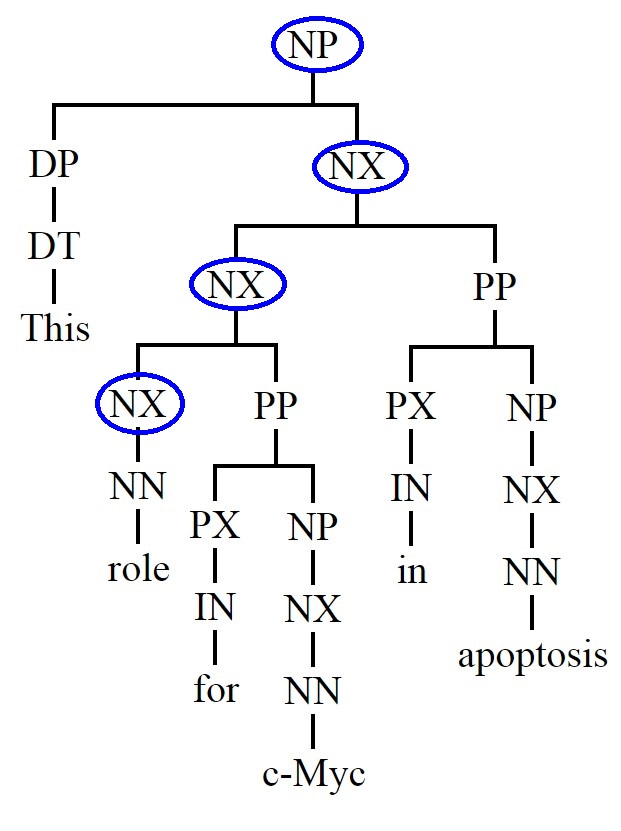
\includegraphics[scale=0.6]{SameHeadWord.jpg} 
 		\caption[Filtering out noun phrases that share the same head word]{ Filtering out noun phrases that share the same head word. In this example, all four noun phrases have the same headword \emph{"role"}. I considered as potential candidate just the longest noun phrases \emph{"This role for c-Myc in apoptosis"}.(In the Enju parser noun phrases are marked with abbreviations NP and NX) }
		\label{Figure 9}
	\end{center}
\end{figure}

Additionally, I did not consider as markables noun phrases that have a subordinate clause in their content (Figure 4.3).

\begin{figure}[h]
	\begin{center}
		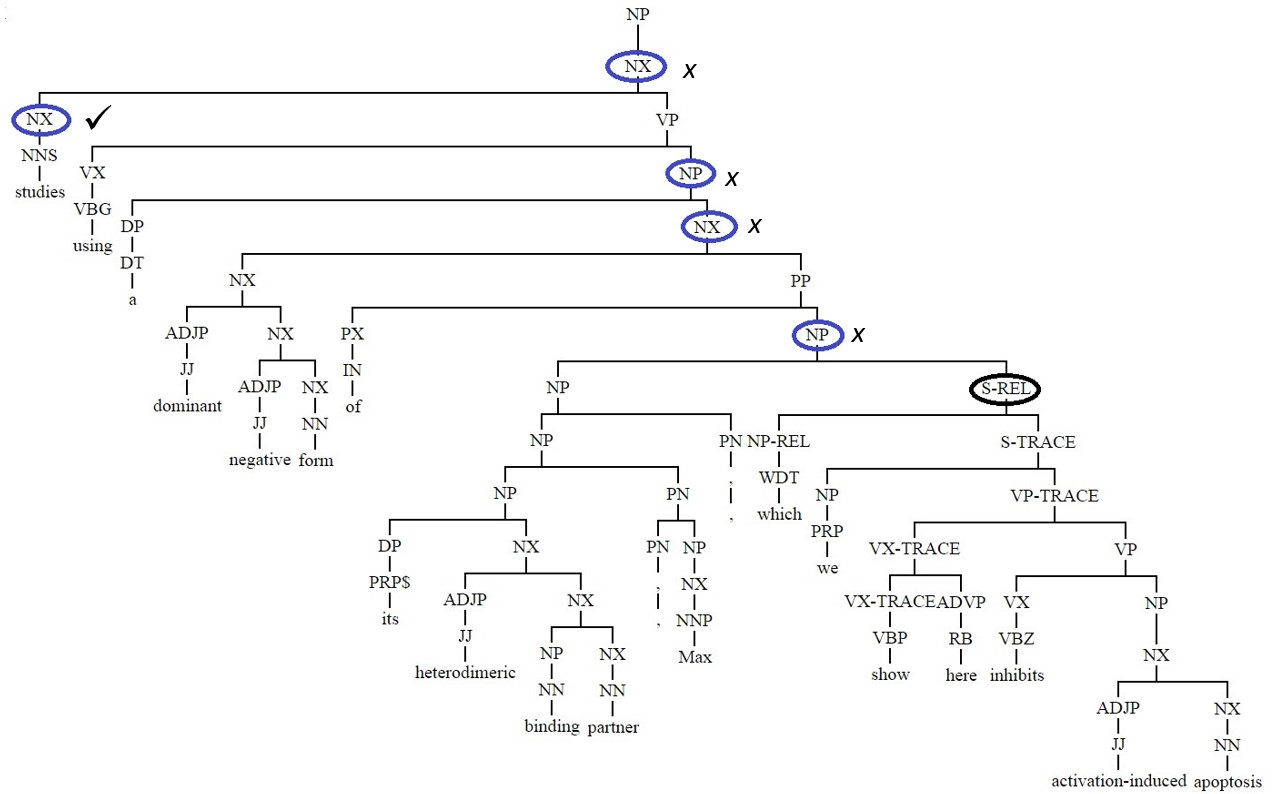
\includegraphics[scale=0.45]{removeSubordinateClause.jpg} 
 		\caption[Filtering out noun phrases that have a subordinate clause in their content]{ Filtering out noun phrases that have a subordinate clause in their content. In this example, I removed noun phrases (marked with \emph{\textbf{x}}) that in their content have the subordinate clause  \emph{"which we show here inhibits activation-induced apoptosis"} }
		\label{Figure 10}
	\end{center}
\end{figure}

\section{Anaphora selection}

\textbf{Anaphora selection} is the step in which I selected text parts that are anaphoric expressions (pronouns and definite noun phrases).
 
I selected the following types of pronouns:

\begin{itemize}
	\item relative pronouns (who, whom, whose, which and that)
	\item personal pronouns (it, they and them)
	\item possessive pronouns (its and their)
	\item definite noun phrases that refer to protein 
\end{itemize}

From the personal pronouns, I just selected the pronouns \emph{"it"} and \emph{"they"} as anaphoric expressions. Other personal pronouns (\emph{I,you,he,she, we and you}) cannot refer to proteins, thus, I filtered and did not select them as anaphoric expressions. Another case of filtering is when the pronoun \emph{"it"} did not refer to any object, for example \emph{"It is important for people to live healthily"}. When the pronoun \emph{"it"} does not refer to an object, it is called \emph{pleonastic}\footnote{ pleonastic (etymology: from Greek word pleonasm which means much, too much) is the phenomena when we use more words than necessary to express a statement to express an idea} \emph{it}. I used patterns to filter pleonastic mentions of the pronoun \emph{it} in similar way like in [3,69]. 

I used these patterns to identify pleonastic it:

\begin{itemize}
	\item \emph{It be $[Adj | Adv | verb]$* that}
	\item \emph{It be Adj $[for NP]$ to VP}
	\item \emph{It $[seems | appears | means | follows]$ that} 
	\item \emph{It has been shown}
\end{itemize}

From possessive pronouns, I only selected the pronouns \emph{its} and \emph{their} as anaphoric expressions. Other possessive pronouns \emph{(my, mine, our, ours, his, her, hers, your, yours)} cannot refer to proteins, thus, I filtered and did not select them as anaphoric expressions.

Identifying anaphoric definite nouns, is a difficult task, because we do not know if a noun phrase is anaphoric or not. In the biomedical domain, many definite nouns do not have an antecedent as the referenced concepts refer to a biomedical entity which is not introduced before or to a general concept. These non-anaphoric expressions appear in scientific texts, because authors assume that the reader has some knowledge in the domain and the authors use the definite noun phrases when they refer to a biomedical entity [3,69]. 

To select the potential anaphoric definite noun phrases, I used semantic knowledge [3,70] and  rules which were generated from the statistics of the corpus. I selected as anaphoric expressions only noun phrases that satisfied the following conditions :

\begin{itemize}
	\item their head noun was protein(s) or gene(s) and start with the words: the, this and these. For example the protein, these two genes and this protein.
	\item their head noun was factor(s), molecule(s), element(s), family, inhibitor(s), receptor(s), complex, construct(s). 
\end{itemize}

Using these filters I covered more than 85\% of the coreference links in the training and the development set.

Indefinite pronouns can act as anaphoric expressions. These cases are not so evident in the biomedical domain. Although these types of expressions are very difficult to identify and my system does not process or try to find these types of anaphoric expressions. In Example 11 the expression "a protein" is an anaphoric expression and its antecedent is "P53". \\
\newpage
\emph{Example (11):}
\begin{changemargin}{10mm}{10mm} 
  \emph{P53, a protein that in humans is encoded by the TP53 gene.}  
\end{changemargin} 
\vspace{4mm}

\subsection{Distribution of anaphoric expressions}
\begin{table}[h]
\centering
   \begin{center}
	 \begin{tabular}{l | C{2cm} C{2cm} C{2cm} C{2cm}}
 		
  		& {\footnotesize BioNLP training data set} & {\footnotesize BioNLP development data set} & {\footnotesize BioNLP test data set} & {\footnotesize Full text data set}\\
 		\hline
 		Relative pronouns & 32\% & 34\% & 26\% & 30\% \\[1.1ex]
 		\hline 
 		Personal pronouns & 10\% & 12\% & 8\% &12\% \\ [1.1ex]
 		\hline   
 		Possessive pronouns & 26\% & 29\% & 31\% &19\% \\ [1.1ex]
 		\hline  
 		Definite noun phrases & 25\% & 19\% & 24\% & 31\% \\[1.1ex]
 		\hline  
 		Other & 7\% & 6\% & 11\% &8\% \\ [1.1 ex]
 		\hline   
	\end{tabular}
  \end{center} 
  \caption{ Distribution of anaphoric expressions that refer to protein by  syntactic category}
\end{table}
  
From Table 4.2, we can see that in \emph{the full text data set} the anaphoric definite noun phrases occurs more often than in abstracts. On the other hand, possessive pronouns occur more often in abstracts than in full text.

\section{Antecedent candidate selection}

In my system, I used rules to resolve pronominal anaphora, rules and  domain dependent features to select the antecedent candidate of a definite noun anaphoric expression. These rules I derived based on the assumption that the subjects of clauses in a complex or a compound sentence  refer to the same object,  and two coordinated noun phrases refer to the same object. To select antecedent candidates for definite noun phrases, I used syntactic structure of the sentences and domain dependant features. Most scientists use the nearest candidate to resolve definite noun anaphoric expressions and also claim that the nearest candidate approach is better than best candidate. In my system I implemented a hybrid approach of nearest first and best first [2,4].

\subsection{Statistics of the data sets}
The first step in antecedent candidates selection of  anaphoric expressions was to find a relationship between antecedents and anaphoras. I measured the distance between an anaphoric expressions and their antecedent. This distance, I measured in sentences as  I wanted to know where to look the antecedent of an anaphoric expression.
 
\begin{table}[h]
   \begin{center}
   \centering
 	  \begin{tabular}{l | C{2cm} C{2cm} C{2cm} C{2cm} @{}m{0pt}@{}}
 		
 		& \multicolumn{4}{c}{Test set}&\\[1.5ex]
 		\hline
 		& D=0 & D=1 & D=2 & D$>$2&\\ [1.1ex]
 		\hline
 		Relative pronouns & 100\% & 0\% & 0\% &0\%& \\ [1.1ex]
 		\hline 
 		Personal pronouns & 80\% & 20\% & 0\% &0\% &\\ [1.1ex]
 		\hline   
 		Possessive pronouns & 83\% & 11\% & 5\% &1\%& \\ [1.1ex]
 		\hline  
 		Definite noun phrases & 31\% & 46\% & 8\% &15\%& \\[1.1ex]	
 		\hline  
 		Other & 47\% & 29\% & 15\% &9\%& \\[1.1 ex]
 		\hline  
  		Total & 72\% & 19\% & 4\% &5\%& \\ [1.1ex]
 		\hline  
     \end{tabular}
   \end{center} 
   \caption{Distribution of anaphoric expressions that refer to protein by category in the \textbf{test set}}
\end{table}

\begin{table}[h]
  \begin{center}
	\begin{tabular}{ l | C{2cm} C{2cm} C{2cm} C{2cm} @{}m{0pt}@{}}
 	    & \multicolumn{4}{c}{Development set}&\\[1.5ex]
 		\hline
 		& D=0 & D=1 & D=2 & D$>$2&\\ [1.1ex]
 		\hline
 		Relative pronouns & 100\% & 0\% & 0\% &0\%& \\ [1.1ex]
 		\hline 
 		Personal pronouns & 84\% & 16\% & 0\% &0\% &\\ [1.1ex]
 		\hline   
 		Possessive pronouns & 90\% & 10\% & 0\% &0\%& \\ [1.1ex]
 		\hline  
 		Definite noun phrases & 42\% & 34\% & 0\% & 8\%& \\ [1.1ex]
 		\hline  
 		Other & 72\% & 14\% & 14\% &14\%& \\ [1.1ex]
 		\hline  
  		Total & 82.6\% & 12.4\% & 1\% &4\%& \\ [1.1ex]
 		\hline  
	\end{tabular}
  \end{center}
  \caption{Distribution of anaphoric expressions that refer to protein by category in the \textbf{development set}}
\end{table}

From these statistics, I decided to use "divide and conquer" techniques to generate the rules and the window size of the search space for each of 4 types (relative pronouns, personal pronouns, possessive pronouns and definite pronouns) of anaphoric expressions.
And the search space for each type is following: 

\begin{itemize}
	\item relative pronouns - window size of one sentence 
	\item personal and possessive pronouns - window size of two sentences
	\item definite nouns window size of three sentences
\end{itemize}

\subsection{Syntax structure of data set}
From the definition of syntax in section 2.2, we saw that syntax is a set of rules and words. This was a good signal that I could use syntax rules to build a coreference resolution system. An important rule from syntax is that anaphora and antecedent should correspond to their number (singular or plural)\footnote{In other domains is important that the antecedent and anaphora to not have different genders.}. 

The Subject-Verb-Object (SVO) structure of declarative sentences in the English language is the most important rule in coreference resolution. This structure can be defined as: "when people express a thought (clause), first they say the subject of the clause (what or whom the sentence is about) then the verb, and in the end the object of the clause".
 
From this property of the English language I derived rules and hypothesis for resolving personal and possessive pronouns. 

I will describe in the following sections  all rules and heuristics that I used in the system.

\subsection{Domain dependent heuristics}
In the section 3.1 (History) we saw that the accuracy of algorithms is dependent from the corpus. Because of this property of coreference resolution systems, I decided to use corpus features in antecedent and anaphora coreference resolution.

I created regular expressions to identify biomedical entities. The regular expression classify every word as biomedical entity, if it contains a capital letter in its content or it contains a number or a special character.

For each definite noun anaphoric expression I select different candidates based on their number (plural or singular) and based on the head noun. I used the following rules to select potential antecedents of a definite noun anaphoric expression:
 
\begin{itemize}
	\item If the anaphoric expression is a \emph{\textbf{plural}} definite noun, and its head word is \emph{\textbf{genes/proteins}} then as potential candidate consider:
	\begin{itemize}
		\item Noun phrases that their head word is genes/proteins 
		\item Noun phrases that their head word is \emph{"family"}
		\item If the previous two rules do not find a potential antecedent candidate then as potential antecedent candidates consider noun phrases that contain 2 or more proteins 
	\end{itemize}
	\item If the anaphoric expression is a \emph{\textbf{singular}} definite noun, and its head word is \emph{\textbf{gene/protein}} then as potential candidate consider:
	\begin{itemize}
		\item Noun phrases that their head word is gene/protein
		\item If the previous rule does not find a potential antecedent candidate then as potential antecedent candidates consider noun phrases that is a protein name 
	\end{itemize}
	\item If the anaphoric expression is a \emph{\textbf{plural}} definite noun, and its head word is \emph{\textbf{inhibitors, elements, complexes, molecules or receptors }} then as potential candidate consider:
	\begin{itemize}
		\item Noun phrases that contain two or more biomedical entities
		\item Noun phrases that have same head word with the anaphoric expression
		\item If the previous two rules do not find a potential antecedent candidate then as potential antecedent candidates consider noun phrases that contain 2 or more proteins 
	\end{itemize}
	\item If the anaphoric expression is a \emph{\textbf{singular}} definite noun, and its head word is \emph{\textbf{inhibitor, element, complex, molecule or receptor }} then as potential candidate consider:
	\begin{itemize}
		\item Noun phrases that have same head word with the anaphoric expression
		\item Noun phrases that contain a biomedical entity
	\end{itemize}
\end{itemize}

\section{Antecedent prediction}
The last step of the coreference resolution process is antecedent selection. For pronoun coreference resolution I have used rules and these rules generate just one candidate. In the definite noun coreference resolution, it is shown in other domains that the nearest potential candidate is the most likely candidate to be the antecedent of the definite noun anaphoric expression. Other methods in selecting the antecedent of an definite noun anaphoric expression were based in choosing the best candidate. The best candidate was selected based in some criteria. All  "best" candidate methods were less accurate than the nearest first. 
 
I created a hybrid method based on nearest candidate first and the "best rules" first. In this hybrid approach, I just select candidates that fulfill the requirements of one the best rules and if these rules find candidates I select the nearest candidate. If these "best rules" do not find a candidate then I run other less accurate rules to find the nearest  antecedent that fulfill one of these less accurate rules.   

\subsection{Relative pronouns}
I realised that relative pronouns and their antecedent are always in the same sentence. Because of this relationship, I measured the distance between the end offset of antecedent and the begin offset of the anaphora. The results were that this distance was less than 5 characters in more than 90\% of relative pronoun anaphora links. These numbers tell us that if we have a relative pronoun then its antecedent is the nearest noun phrase.

\begin{figure}[h]
  \begin{center}
	 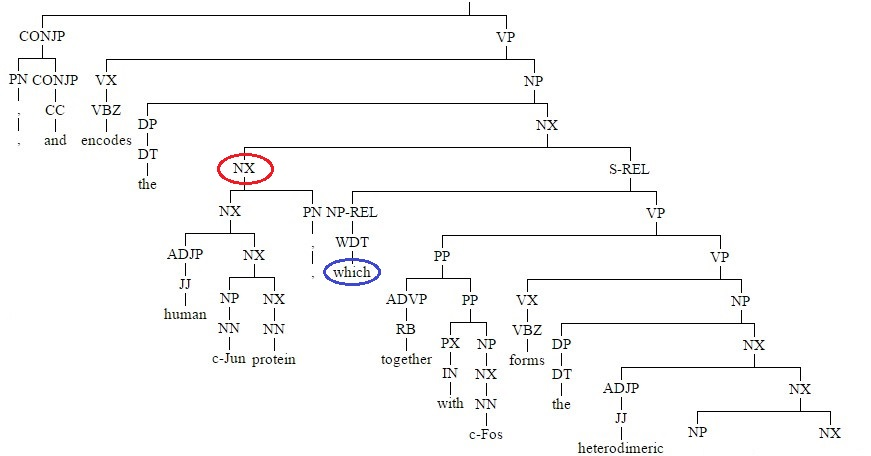
\includegraphics[scale=0.6]{relative.jpg} 
 	 \caption[Coreference resolution of relative pronouns]{Coreference resolution of relative pronouns}
	 \label{Figure 11}
  \end{center}
\end{figure}
 
\subsection{Personal pronouns} 
From the statistics and mining the data set I realised that when  the personal pronoun appears in the second or third clause of the sentence then its antecedent is the  subject of the previous (nearest) clause, in the first or in the second clause, respectively.  The same rule is when in the sentence we have two coordinated noun phrases. 

If the personal pronoun appears in the first clause then the personal pronoun is the subject of the sentence. In this case, I take as antecedent the subject of the previous  sentence.

\begin{figure}[h]
  \begin{center}
	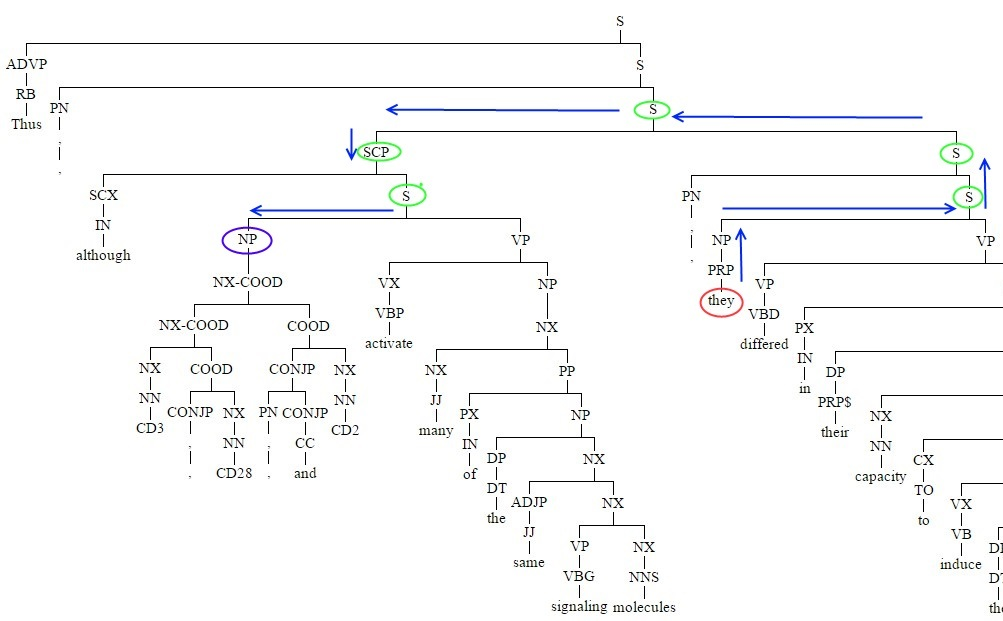
\includegraphics[scale=0.53]{PersonalPronounsNP.jpg} 
 	\caption[Simulation of  a rules in personal pronouns]{Simulation of  the rule when the anaphora is in the second clause and the antecedent is in the first clause of a complex sentence.}
	\label{Figure 12}
  \end{center}
\end{figure}

\footnotetext{Sentence "Thus, although CD3, CD28, and CD2 activate many of the same signaling molecules, they differed in their capacity to induce the tyrosine phosphorylation of HSI." is taken from PMID-9794375}

An exception is when we have two coordinated verb phrases. If  the anapha (it or they) appears in a coordinated verb phrase, and it is in the second verb phrase, then I do not search for antecedent in the first verb phrases because "the verb phrase describe an activity that is taken from the subject". Thus, both verb phrases of coordinated phrases describe an activity, and the activity is taken by the subject of the sentence and I select as antecedent the subject of previous clause (sentence) in which the anaphora appears. 
\newpage
\begin{figure}[h]
  \begin{center}
	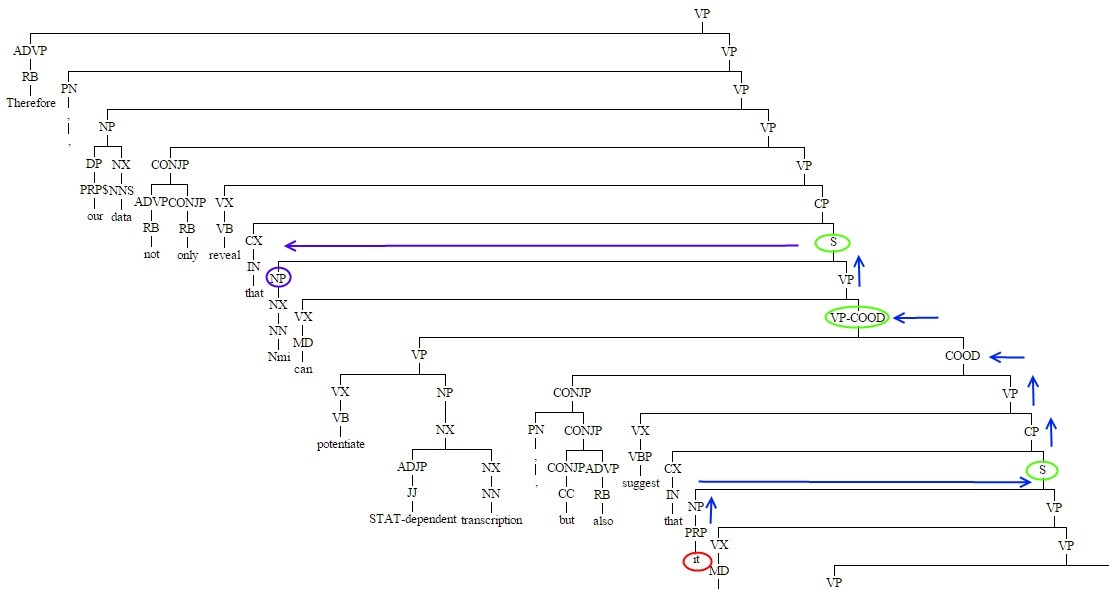
\includegraphics[scale=0.50]{PersonalPronounsVP.jpg} 
 	\caption[Simulation of  a rules in personal pronouns]{Simulation of  the rule when the anaphora is in the second verb phrase of a coordinated verb phrase and I chose as antecedent the subject of the nearest clause (sentence).\footnotemark}
	\label{Figure 13}
  \end{center}
 \end{figure}
 
\footnotetext{Sentence "Therefore, our data not only reveal that Nmi can potentiate STAT-dependent transcription, but also suggest that it can augment co-activator protein recruitment to at least some members of a group of sequence-specific transcription factors." is taken from PMID-8108414}


\subsection{Possessive pronouns}

The same idea and the same rules I applied in possessive pronouns. From the mining of the corpus,I realised that possessive pronouns appear more in coordinated noun phrases. 
\newpage
\begin{figure}[h]
  \begin{center}
	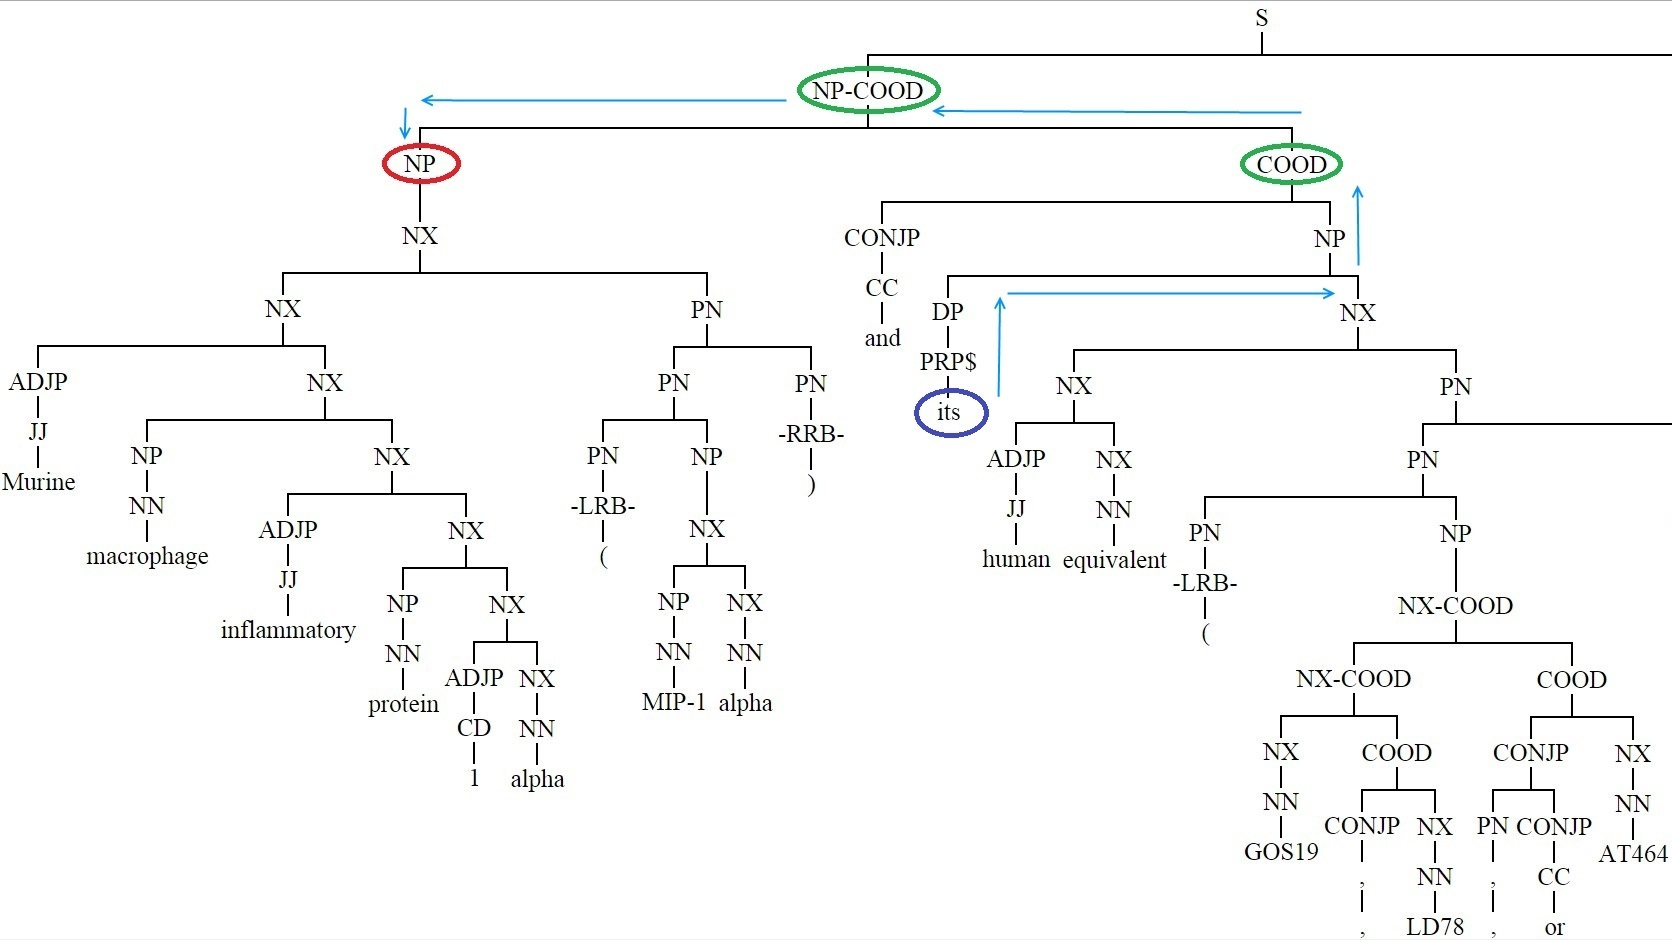
\includegraphics[scale=0.30]{PossesiveNP.jpg} 
 	\caption[Simulation of  a rules in possessive pronouns]{Simulation of  the rule when the anaphora  is in the second coordinated noun phrase of a coordinated noun phrase and I chose the antecedent from the previous noun phrase\footnotemark}
	\label{Figure 14}
  \end{center}
 \end{figure}
 
\footnotetext{Sentence "Therefore, our data not only reveal that Nmi can potentiate STAT-dependent transcription, but also suggest that it can augment coactivator protein recruitment to at least some members of a group of sequence-specific transcription factors." is taken from PMID-8108414}
\newpage

\begin{figure}[h]
  \begin{center}
	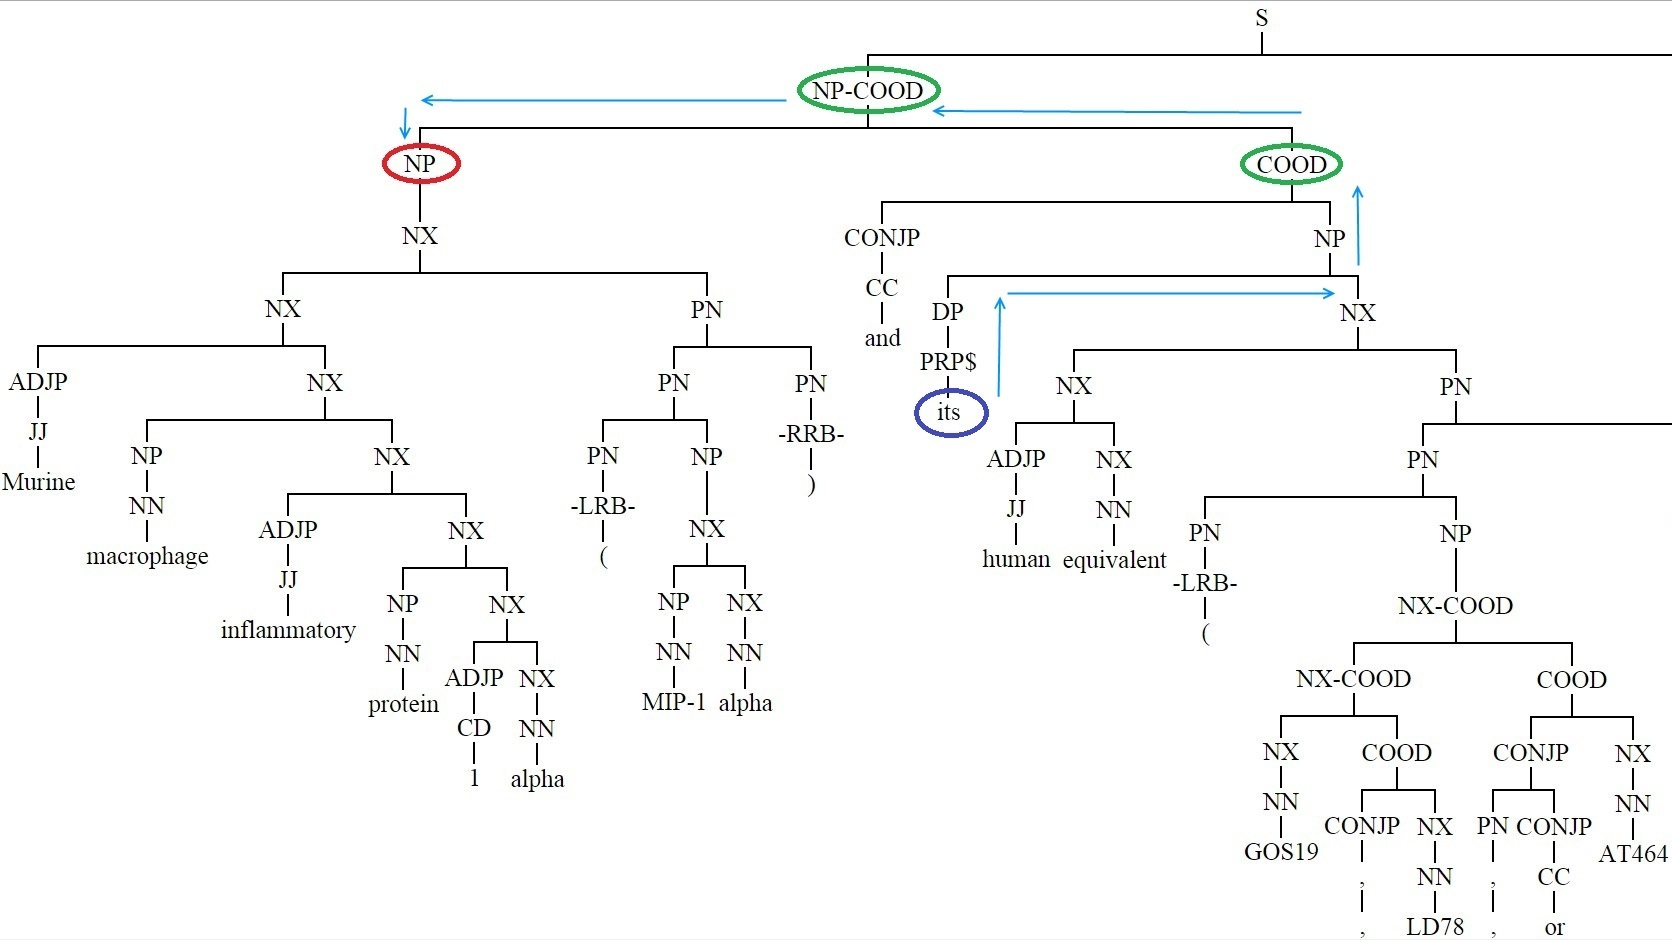
\includegraphics[scale=0.30]{PossesiveNP.jpg} 
 	\caption[Simulation of  a rules in possessive pronouns]{Simulation of  the rule when the anaphora  is in the second coordinated noun phrase of a coordinated noun phrase and I chose the antecedent from the previous noun phrase\footnotemark}
	\label{Figure 15}
  \end{center}
\end{figure}

\footnotetext{Sentence "Murine macrophage inflammatory protein 1 alpha (MIP-1 alpha) and its human equivalent (GOS19, LD78, or AT464) are members of the -C-C family of low-molecular-weight chemokines." is taken from PMID-7760807}

\subsection{Definite noun phrases} 

I select the nearest candidate of the candidates that fulfill the requirements of the "best" rules, then if there is no candidate selected then I run the other rules to select the nearest noun phrase that fulfill the requirements of the less accurate rules.  

		\chapter{Results}
\label{Results}
\section{Results}

In this chapter I will show the performance results for the protein coreference resolution system.The evaluation is done in the way that is described in the first chapter. To evaluate the system in the development and the test set I used the BioNLP online testing system [71,72]. In the development set there are 202 coreferent links the system should predict and in the test set there are 284 coreferent links that the system should predict.  

I will show the result of the whole system and I will compare with the current state of the art method and other best methods.

For the development data set I will compare results with current state of the art methods in each of 4 types (personal,possessive, relative and definite noun phrases). 

Additionally, I will present the first result in 243 coreferent link in coreference resolution in full text articles.

\begin{table}[h]
\centering
   \begin{center}
	 \begin{tabular}{l | C{1.7cm} C{2cm} C{1.7cm} @{}m{0pt}@{}}
 		
  		Methods & Recall & Precision & F &  \\[1.1ex]
 		\hline
 		CR resolver & 52.5 & 50.2 & 51.3&  \\ [1.1ex]
 		\hline 
 		Current state of the art & 55.6 & 67.2 & 60.9 & \\ [1.1ex]
 		\hline   
 		\textbf{My system} & \textbf{60.92} & \textbf{65.53} & \textbf{63.14}& \\ [1.1ex]
 		\hline  
 	\end{tabular}
  \end{center} 
  \caption{ Results on the test set of the current best methods and my system }
\end{table}
Table 5.1 shows the result of the system and the current state of the art algorithms in Protein coreference resolution in the test data set. The evaluation measures precision (P), recall (R), and F-measure (F)  are in presented in percentage. The system performance is tested in the online system of the Protein coreference task website. This test is performed in the test data set which consists of 250 documents and in this data set appear 284 protein coreference links. The new methods that I implemented in the system improved for 5.3\% the recall and doped the precision for 1.7\%. My system outperforms the current state of the art  method in the F-measure by 2.24\%.

The table 5.2 shows the result of the system in the full text. The system performance is tested in 8 full text documents, in which appear 243 protein coreference links. The result that I present in this thesis are first results in full text articles. This results are first because the protein coreference  resolution is a new research filed and  does not exist an annotated corpus with full text articles.   
\begin{table}[h] 
   \begin{center}
	 \begin{tabular}{l | C{1.7cm} C{2cm} C{1.7cm}  @{}m{0pt}@{} }
 		
  		Methods & Recall & Precision & F1 & \\ [1.1ex]
 		\hline
 		\textbf{My system} & \textbf{61.3} & \textbf{82.3} & \textbf{70.2}& \\ [1.1ex]
 		\hline  
 	\end{tabular}
  \end{center} 
  \caption{Results of the coreference resolution system on full text articles}
\end{table}

\begin{table}[h]
   \begin{center}
   {
   \centering
	 \begin{tabular}{L{3.5cm} | C{0.8 cm} C{0.8cm} C{0.8cm} | C{0.8cm} C{0.8cm} C{0.8cm} | C{1.25cm}}
	 & \multicolumn{3}{c|}{{\footnotesize Current state of the art}} & \multicolumn{3}{c|}{{\footnotesize My system}}\\
	 \hline
 		& {\footnotesize R} & {\footnotesize P} & {\footnotesize F} & {\footnotesize R} & {\footnotesize P} & {\footnotesize F} &  {\footnotesize Diff. } \\
 		\hline
 		{\footnotesize Relative pronouns} & {\footnotesize 83.8} & {\footnotesize 83.8} & {\footnotesize \textbf{83.8}} & {\footnotesize 85.3} & {\footnotesize 78.4} & {\footnotesize \textbf{81.7}} & {\footnotesize \textcolor{red}{\textbf{-2.1}}} \\
 		\hline 
 		{\footnotesize Per. \& poss. pronouns} & {\footnotesize 63.8} & {\footnotesize 77.9} & {\footnotesize \textbf{70.2}} & {\footnotesize 75.6} & {\footnotesize 74.7} & {\footnotesize \textbf{75.1}} & {\footnotesize \textcolor{blue}{\textbf{+4.9}}} \\
 		\hline   
 		{\footnotesize Definite noun phrases} & {\footnotesize 36.8} & {\footnotesize 58.3} & {\footnotesize \textbf{45.2}} & {\footnotesize 45.2} & {\footnotesize 66.7} & {\footnotesize \textbf{55.4}} & {\footnotesize\textcolor{blue}{\textbf{ +10.2}}} \\
 		\hline  
 		{\footnotesize Whole system} & {\footnotesize 59.9} & {\footnotesize 77.1} & {\footnotesize \textbf{67.4}} & {\footnotesize 68.3} & {\footnotesize 75} & {\footnotesize \textbf{71.5}} & {\footnotesize \textcolor{blue}{\textbf{+4.1}}} \\
 		\hline  
 	\end{tabular}
 	}
  \end{center} 
    \caption{ Results on the development set of the current best methods and my system }
\end{table}
\section{Discussion}
The developed rules which model the relationship between subjects of clauses in the sentence and coordinated phrases, bring significant improvement of more than 4\% in F-score. An improvement of more than 10\% is in the definite noun phrase protein coreference resolution. The new method, which first evaluate the best methods and then predict the nearest candidate as antecedent, and the domain syntactic and domain features had a huge impact in the improvement of the result.  In the other hand,rules gave a decline in for more than 2\% in relative pronouns. Also, I have to say that this system can not achieve an recall better than 92\%, because the system does not resolve the anaphoric indefinite noun phrase expressions. 

In the full text articles system achieves 70.2\% F-score. The system achieves higher precision in full text than in abstracts but lower recall. These differences in precision and recall  of the system in two different data sets are because coreference resolution algorithms are sensitive and dependent from the corpus.
		
		
		% ---------------------------------------------------------------------------
		%
		% Appendix
		%
		% ---------------------------------------------------------------------------
		
		
		
		%\appendix %---------------------------------------
		\listoftables
		\newpage
		\listoffigures
	

	
  \clearemptydoublepage
 
	\bibliography{bibliography/literature}
	\chapter{Bibliography}
\label{Bibliography}
$\big[1\big]$ Ngan Nguyen, Jin-Dong Kim and Jun'ichi Tsujii. Overview of the Protein Coreference task in BioNLP Shared Task 2011.\emph{In Proceedings of BioNLP Shared Task 2011 Workshop}, pages 74-82 Portland, Oregon, USA, 24 June, 2011.  2011 Association for Computational Linguistics\\  \\ 
\big[2\big] Xiaofeng Yang, Jian Su, and Chew Lim Tan. 2004a Improving noun phrase coreference resolution by matching strings. \emph{In Proceedings of the First International Joint Conference on Natural Language Processing}, pages 22-31.\\  \\
\big[3\big] Ngan Nguyen, Jin-Dong Kim, Makoto Miwa, Takuya Matsuzaki and Jun'ichi Tsujii. Improving protein coreference resolution by simple semantic classification. November 2012 BMC Bioinformatics, 13:304\\  \\
\big[4\big] Wee Meng Soon, Hwee Tou Ng, and Daniel Chung Yong Lim. A machine learning approach to coreference resolution of noun phrases 2001. \emph{Computational linguistics}, 27(4):521-544\\  \\
\big[5\big] Yannick Versley, Simone Paolo Ponzetto, Massimo Poesio, Vladimir Eidelman, Alan Jern, Jason Smith, Xiaofeng Yang, and Alessandro Moschitti. 2008b. BART: A modular toolkit for coreference resolution. \emph{In Proceedings of the ACL-08: HLT Demo Session}, pages 9-12.\\  \\
\big[6\big]Laura Hasler, Constantin Orasan, and Karin Naumann.2006. NPs for events: Experiments in coreference annotation. \emph{In Proceedings of the 5th International Conference on Language Resources and Evaluation,} pages 1167-1172.\\  \\
\big[7\big] Jin-Dong Kim, Sampo Pyysalo,Tomoko Ohta,Robert Bossy, Ngan Nguyen,Jun'ichi Tsujii Overview of BioNLP Shared Task 2011, \emph{In Proceedings of BioNLP Shared Task 2011 Workshop}, pages 1-6 Portland, Oregon, USA, 24 June, 2011.  2011 Association for Computational \\  \\
\big[8\big]   Ronen Feldman and James Sanger.The Text Mining Handbook:  Advanced Approaches in Analyzing Unstructured Data.   Cambridge University Press, Cam-bridge, MA, USA, December 2006.\\  \\
\big[9\big]  Fabio Celli and Massimo Poesio. Improving Relation Extraction with Anaphora In Italian DAARC 2011\\  \\
\big[10\big] M.Novak. Utilization of Anaphora in Machine Translation in \emph{WDS 2011 Proceedings of Contributed Papers: Part I, ser}. WDS 11, 2011, pages. 155 - 160.WDS'11 Proceedings of Contributed Papers, Part I, 155-160, 2011 \\  \\
\big[11\big] Christian Hardmeier and Marcello Federico. 2010. Modeling Pronominal Anaphora in Statistical Machine Translation. \emph{In International Workshop on Spoken Language Translation (IWSLT)}, Paris, December 2nd and 3rd, 2010, pages 283 -289\\  \\
\big[12\big] Ruslan Mitkov ,Sung-Kwon Choi and Randall Sharp. ANAPHORA RESOLUTION IN MACHINE TRANSLATION in \emph{Proceedings of the Sixth International Conference on Theoretical and Methodological Issues in Machine Translation}, pages 87-98 \\  \\
\big[13\big] Liddy, E.D. Natural Language Processing. \emph{In Encyclopedia of Library and Information Science, 2nd} Ed. NY. Marcel Decker, Inc. 2001\\  \\
\big[14\big] Gobinda G Chowdhury. Natural language processing,2003. \emph{In Annual review of information science and technology} vol 37, pages 51-89\\  \\
\big[15\big]  Sætre, Rune, Kazuhiro Yoshida, Akane Yakushiji, Yusuke Miyao, Yuichiro Matsubayashi and Tomoko Ohta. AKANE System: Protein-Protein Interaction Pairs in BioCreAtIvE2 Challenge, PPI-IPS subtask. \emph{In Proceedings of the Second BioCreative Challenge Evaluation Workshop}, pages 209-212, April 2007. CNIO. \\  \\
\big[16\big] Joseph Olive, Caitlin Christianson, and John McCary. 2011.\emph{Handbook of Natural Language Processing and Machine Translation: DARPA Global Autonomous Language Exploitation}. Springer Publishing Company, Inc., 1st edition.(page 97) \\  \\
\big[17\big] Huihsin Tseng, Pichuan Chang, Galen Andrew, Daniel Jurafsky and  Christopher Manning. A conditional random field word segmenter for sighan bakeoff 2005,  \emph{In Proceedings of the Fourth SIGHAN Workshop on Chinese Language Processing}, pages 168-171, Jeju Island, Korea.\\  \\
\big[18\big] Pi-Chuan Chang, Michel Galley, and Christopher D. Manning. Optimizing Chinese Word Segmentation for Machine Translation Performance 2008  \emph{in Proceedings of the Third Workshop on Statistical Machine Translation}, pages 224-232 \\  \\
\big[19\big] Hai Zhao, Chang-Ning Huang and Mu Li An. Improved Chinese Word Segmentation System with Conditional Random Field  in \emph{Proceedings of the Fifth SIGHAN Workshop on Chinese Language Processing} 2006, pages 162-165, Sydney.\\ \\
\big[20\big] Manabu Sassano. An empirical study of active learning with support vector machines for japanese word segmentation. \emph{In Proceedings of the 40th Annual Meeting of the Association for ComputationalbLinguistics}, pages 505-512, 2002 \\ \\
\big[21\big] Josef Steinberger , Massimo Poesio Mijail A. Kabadjov and  Karel Jezek. Two uses of anaphora resolution in summarization in \emph{ J. Steinberger et al.Information Processing and Management} 43 (2007), pages 1663-1680 \\  \\
\big[22\big] Ruslan Mitkov, Richard Evans, Constantin Orasan, Le An Ha, and Viktor Pekar. Anaphora Resolution: To What Extent Does It Help NLP Applications?  DAARC 2007, LNAI 4410, pages. 179-190, 2007\\  \\
\big[23\big] Heeyoung Lee, Angel Chang, Yves Peirsman, Nathanael Chambers, Mihai Surdeanu, and Dan Jurafsky (2013). Deterministic coreference resolution based on entity-centric, precision-ranked rules. \emph{Computational Linguistics}, pages 1-54, January 2013. 
\big[24\big] Kees van Deemter and Rodger Kibble. 2000. On coreferring: Coreference in MUC and related annotation schemes. \emph{Computational Linguistics,} 26(4):629-637. Squib \\  \\
\big[25\big] Marco Maggini, Natural Language Processing Part 3: Syntax  grammar chunking  constituents   \\  \\
\big[26\big] Jirka Hana. Intro to Linguistics - Syntax 1, November 7, 2011 \\  \\
\big[27\big] Jean Eggenschwiler and Emily Dotson. Cliffs Quick Review Writing: Grammar, Usage, and Style Paperback - May 29, 2001 by Jean Eggenschwiler  (Author), Emily Dotson Biggs (Author) \\  \\
\big[28\big] Andrew Radford. An Introduction to English Sentence Structure, Cambridge, 2004, ISBN-13 978-0-511-50666-6 \\  \\
\big[29\big] Andrew Carnie. Syntax,,Oxford (2001)\\  \\
\big[30\big] Adrian Brasoveanu Anaphora Resolution Spring 2010, UCSC - \\  \\
\big[31\big] Massimo Poesio, Simone Ponzetto, and Yannick Versley. 2011. Computational models of anaphora resolution:A survey. Unpublished. \\  \\
\big[32\big] Xiaofeng Yang, Jian Su, Jun Lang, Chew Lim Tan, and Sheng Li. 2008a. An entity-mention model for coreference resolution with inductive logic programming. \emph{In Proceedings of ACL-08: HLT}, pages 843-851.\\  \\
\big[33\big] Yimeng Zhang and  Yangbo Zhu. Machine Learning for Coreference Resolution: Recent Developments \\  \\
\big[34\big] Shumin Wu and Nicolas Nicolov. Coreference Resolution, A Machine Learning Approach  \\  \\
\big[35\big] Pradheep Elango. Coreference Resolution: A Survey,Technical Report, University of Wisconsin Madison.  \\  \\
\big[36\big] Hannaneh Hajishirzi Leila Zilles Daniel S. Weld Luke Zettlemoyer. Joint Coreference Resolution and Named-Entity Linking with Multi-pass Sieves.   \emph{In proceeding Conference on Empirical Methods on Natural Language Processing}, pages 289-299. ACL. \\  \\
\big[37\big] Hoifung Poon and Pedro Domingos. 2008. Joint unsupervised coreference resolution with Markov logic. \emph{In Proceedings of the 2008 Conference on Empirical Methods in Natural Language Processing}, pages 649-658, Honolulu, HI. ACL. \\  \\
\big[38\big] Shasha Liao and Ralph Grishman. Large Corpus-based Semantic Feature Extraction for Pronoun Coreference. \emph{ In Proceedings 23rd International Conference on Computational}  pages 60-68 \\  \\
\big[39\big] Ruslan Mitkov. 1999. Anaphora resolution: The state of the art. Technical Report (Based on the COLING/ACL-98 tutorial on anaphora resolution), University of Wolverhampton, Wolverhampton. \\  \\
\big[40\big] Fredrik Olsson. A Survey of Machine Learning for Reference Resolution in Textual Discourse. Technical report, Swedish Institute of Computer Science, Kista, 2004.\\  \\
\big[41\big] Aria Haghighi and Dan Klein. 2009. Simple Coreference Resolution with Rich Syntactic and Semantic Features. In Proceedings of the 2009 Conference on Empirical Conference in Natural Language Processing.\\  \\
\big[42\big] Delip Rao and Paul McNamee and Mark Dredze. Streaming cross document entity coreference resolution. \emph{In: Conference on Computational Linguistics (COLING) (2010)} \\  \\
\big[43\big] Rahman Altaf and Vincent Ng. 2009.Supervised models for coreference resolution. \emph{ In Proceedings of the 2009 Conference on Empirical Methods in Natural Language Processing (EMNLP)}, pages 968-977, Suntec. Vincent Ng \\  \\
\big[44\big] David Bean and Ellen Riloff. 2004. Unsupervised learning of contextual role knowledge for coreference resolution. \emph{ In Proceedings  of HLT/NAACL}, pages 297-304. \\  \\
\big[45\big] Unsupervised Models for Coreference Resolution, Vincent Ng \\  \\
\big[46\big] Hobbs, Jerry R., 1976. Pronoun Resolution.  Research Report 76-1, Department of Computer Sciences, City College, City University of New York. August 1976.  \\  \\
\big[47\big] Hobbs, Jerry R., 1978, "Resolving Pronoun References", Lingua, Vol.  44, pp. 311-338.  Also in Readings in Natural Language Processing, B. Grosz, K. Sparck-Jones, and B. Webber, editors, pp. 339-352, Morgan Kaufmann Publishers, Los Altos, California. (a shorter version of the original) \\  \\
\big[48\big] Grosz, Barbara. J., Aravind. K. Joshi, and Scott Weinstein. 1995. Centering: A framework for modeling the local coherence of discourse. \emph{Computational Linguistics}, 21(2):202-225. (The paper originally appeared as an unpublished manuscript in 1986.). \\  \\
\big[49\big] Gasperin Statistical anaphora resolution Caroline Gasperin and Ted Briscoe \emph{in Proceedings of the 22nd International Conference on Computational Linguistics (Coling 2008)} pages 257-264, Manchester , August 2008 \\  \\ 
\big[50\big] http://www.nactem.ac.uk/enju/ Enju parser \\  \\
\big[51\big] Yusuke Miyao and Jun'ichi Tsujii. 2002. Maximum Entropy Estimation for Feature Forests. \emph{In Proceedings of HLT 2002}.\\  \\
\big[52\big] Yusuke Miyao and Jun'ichi Tsujii. 2003. Probabilistic modeling of argument structures including non-local dependencies. \emph{In Proceedings of the Conference on Recent Advances in Natural Language Processing (RANLP)} 2003, pages, 285-291 \\  \\
\big[53\big] Yusuke Miyao, Takashi Ninomiya, and Jun'ichi Tsujii. 2004. Corpus-oriented Grammar Development for Acquiring a Head-driven Phrase Structure Grammar from the Penn Treebank. In Proceedings of IJCNLP-04.\\  \\
\big[54\big] Yusuke Miyao and Jun'ichi Tsujii. 2005. Probabilistic Disambiguation Models for Wide-Coverage HPSG Parsing. \emph{In Proceedings of ACL-2005}, pages. 83-90.\\  \\
\big[55\big] http://www.nactem.ac.uk/y-matsu/geniass/ Genia sentence splitter\\  \\
\big[56\big] Takashi Ninomiya, Takuya Matsuzaki, Yoshimasa Tsuruoka, Yusuke Miyao and Jun'ichi Tsujii. 2006. Extremely Lexicalized Models for Accurate and Fast HPSG Parsing. \emph{In Proceedings of EMNLP 2006.}\\  \\
\big[57\big] Takashi Ninomiya, Takuya Matsuzaki, Yusuke Miyao, and Jun'ichi Tsujii. 2007. A log-linear model with an n-gram reference distribution for accurate HPSG parsing. \emph{In Proceedings of IWPT 2007}.\\  \\
\big[58\big] Yusuke Miyao and Jun'ichi Tsujii. 2008. Feature Forest Models for Probabilistic HPSG Parsing. \emph{Computational Linguistics.} 34(1), pages 35-80, MIT Press.\\  \\
\big[59\big] http://www.nactem.ac.uk/y-matsu/geniass/ genia sentence spliter\\  \\
\big[60\big] Sætre, Rune, Kazuhiro Yoshida, Akane Yakushiji, Yusuke Miyao, Yuichiro Matsubayashi and Tomoko Ohta., AKANE System: Protein-Protein Interaction Pairs in BioCreAtIvE2 Challenge, PPI-IPS subtask.\emph{In Proceedings of the Second BioCreative Challenge Evaluation Workshop}. pages. 209-212, April 2007. CNIO. \\  \\
\big[61\big] Yoshimasa Tsuruoka., A simple C++ library for maximum entropy classification, http://www-tsujii.is.s.u-tokyo.ac.jp/~tsuruoka/maxent/ , .\\  \\
\big[62\big] Jin-Dong Kim, Tomoko Ohta, Yuka Tateishi, and Jun'ichi Tsujii. 2003. GENIA corpus - a semantically annotated corpus for bio-textmining. \emph{Bioinformatics, 19(Suppl.1)}:180-182. \\  \\
\big[63\big]http://2011.bionlp-st.org/ bionlp shared task 2011\\  \\
\big[64\big] Miji Choi, Karin Verspoor and Justin Zobel.2014. Evaluation of coreference resolution for biomedical text.\emph{In proceeding of MedIR 2014, page 2.} \\ \\
\big[65\big]  Yannick Versley, Alessandro Moschitti, Massimo Poesio and Xiaofeng Yang.2008. Coreference systems based on kernel methods. \emph{In Proceedings of COLING}, pages 961-968.\\  \\
\big[66\big] Ninomiya, Takashi, Yoshimasa Tsuruoka, Yusuke Miyao, and Jun'ichi Tsujii. 2005. Efficacy of beam thresholding, unification filtering and hybrid parsing in probabilistic HPSG parsing. \emph{In Proceedings of the 9th International Workshop on Parsing Technologies}, pages 103-114, Vancouver \\  \\
\big[67\big] www.tagtog.net \\  \\
\big[68\big] Cejuela,J.M., McQuilton,P., Ponting,L. et al. tagtog: interactive and text-mining-assisted annotation of gene mentions in PLOS full-text articles. Database (2014) Vol. 2014: article ID bau033; doi:10.1093/database/bau033. \\  \\
\big[69\big] Yu hsiang Lin and Tyne Liang. 2004. Pronominal and sortal anaphora resolution for biomedical literature. \emph{In In Proceedings of ROCLING XVI: Conference on Computational Linguistics and Speech Processing}. \\  \\
\big[70\big] Jennifer D'Souza and Vincent Ng. Anaphora Resolution in Biomedical Literature: A Hybrid Approach. \emph{In Proceeding of BCB '12 Proceedings of the ACM Conference on Bioinformatics}, Computational Biology and Biomedicine Pages 113-122 \\  \\
\big[71\big] http://bionlp-st.dbcls.jp/CO/eval-test/\\  \\
\big[72\big] http://bionlp-st.dbcls.jp/CO/eval-development/\\  \\
\big[73\big] Mitkov, Ruslan. 2002. Anaphora Resolution. London: Pearson Longman.\\  \\



	
 
\end{document}

